\documentclass[a4paper, 12pt]{article}
\usepackage[letterpaper, top=2.5cm, bottom=2.5cm, left=3cm, right=3cm]{geometry} %margenes
\usepackage{fancyhdr} %formato de los encabezados de página
\pagestyle{fancy} %estilo
\fancyhf{}
\fancyhead[L]{\textbf{Fundamentos de Bases de Datos}} %encabezado Esquina Superior Izquierda
\fancyhead[R]{\textbf{Proyecto final}} %encabezado Esquina Superior Derecha
\fancyfoot[R]{\thepage}
\usepackage[utf8]{inputenc} %manejo de caracteres especiales
\usepackage[spanish]{babel} %manejo de encabezados de inglés a español
\usepackage{ragged2e} %alineado real justficado
\usepackage{graphicx} %manejo de imagenes
\usepackage{amsmath} %manejo de notación matemática
\usepackage{mathtools} %manejo de notación matemática
\usepackage{blindtext} %texto de relleno
\usepackage{amssymb} %manejo de simbología
\usepackage{float} %centrado de imaene
\usepackage{hyperref} %manejo de enlaces e hipervínculos
\usepackage{enumerate}

\hypersetup{
  colorlinks   = true, %Colours links instead of ugly boxes
  urlcolor     = black, %Colour for external hyperlinks
  linkcolor    = black, %Colour of internal links
  citecolor   = black %Colour of citations
}

\begin{document}
    
    %PORTADA
    \begin{titlepage}
        \begin{figure}[ht]
            \centering
            
\includegraphics[width=15cm]{logosITT.png}
        \end{figure}
        \centering
        {\scshape\LARGE Tecnológico Nacional de México\\Instituto Tecnológico de Tijuana\par}
        \vspace{1cm}
        {\scshape\Large Fundamentos de Bases de Datos\par}
        \vspace{1cm}
        {\scshape\Large Unidad 6\par}
        \vspace{1.5cm}
        {\huge\bfseries Proyecto Final\par}
        \vspace{2cm}
        {\Large\itshape C. Abraham Jhared Flores Azcona\\19211640\par}
        \vfill
        Profesora: \par
        M.C. María Magdalena Serrano Ortega
    
        \vfill

        {\large 25 de junio de 2021}
    \end{titlepage}

    %indices
    \newpage
        \pagestyle{empty}
        \tableofcontents %indice de contenidos

    %cuerpo
    \newpage
    \begin{justify}
        \setcounter{page}{1}
        \pagestyle{fancy}
        \section*{Introducción}
        \justify
        En este proyecto, se hace un compendio de 4 trabajos realizados con anterioridad en la materia para ser transcritos a SQL como
        Introducción al mismo y para concluír lo visto en la materia.
        \\\newline
        Se muestra el escrito del problema, su diagrama entidad-relación realizado para dicha actividad, el código de la consulta de SQL y el
        diagrama generado por SQL.
        \section{Actividad: Notación UML}
        \subsection{Ejercicio 1}
        \justify
        A partir del siguiente enunciado se desea realizar el modelo entidad-relación.
        ``Una empresa vende productos a varios clientes. Se necesita conocer los datos personales de los clientes
        (nombre, apellidos dni, dirección y fecha de nacimiento). Cada producto tiene un nombre y un código, así como un precio
        unitario. Un cliente puede comprar varios clientes. Los productos son suministrados por diferentes proveedores.
        Se debe tener en cuenta que un producto sólo puede ser suministrado por un proveedor, y que un proveedor puede
        suministrar diferentes productos. De cada proveedor se desea conocer el NIF, nombre y dirección.''
        \subsubsection{Diagrama E-R}
        \begin{figure}[H]
            \centering
            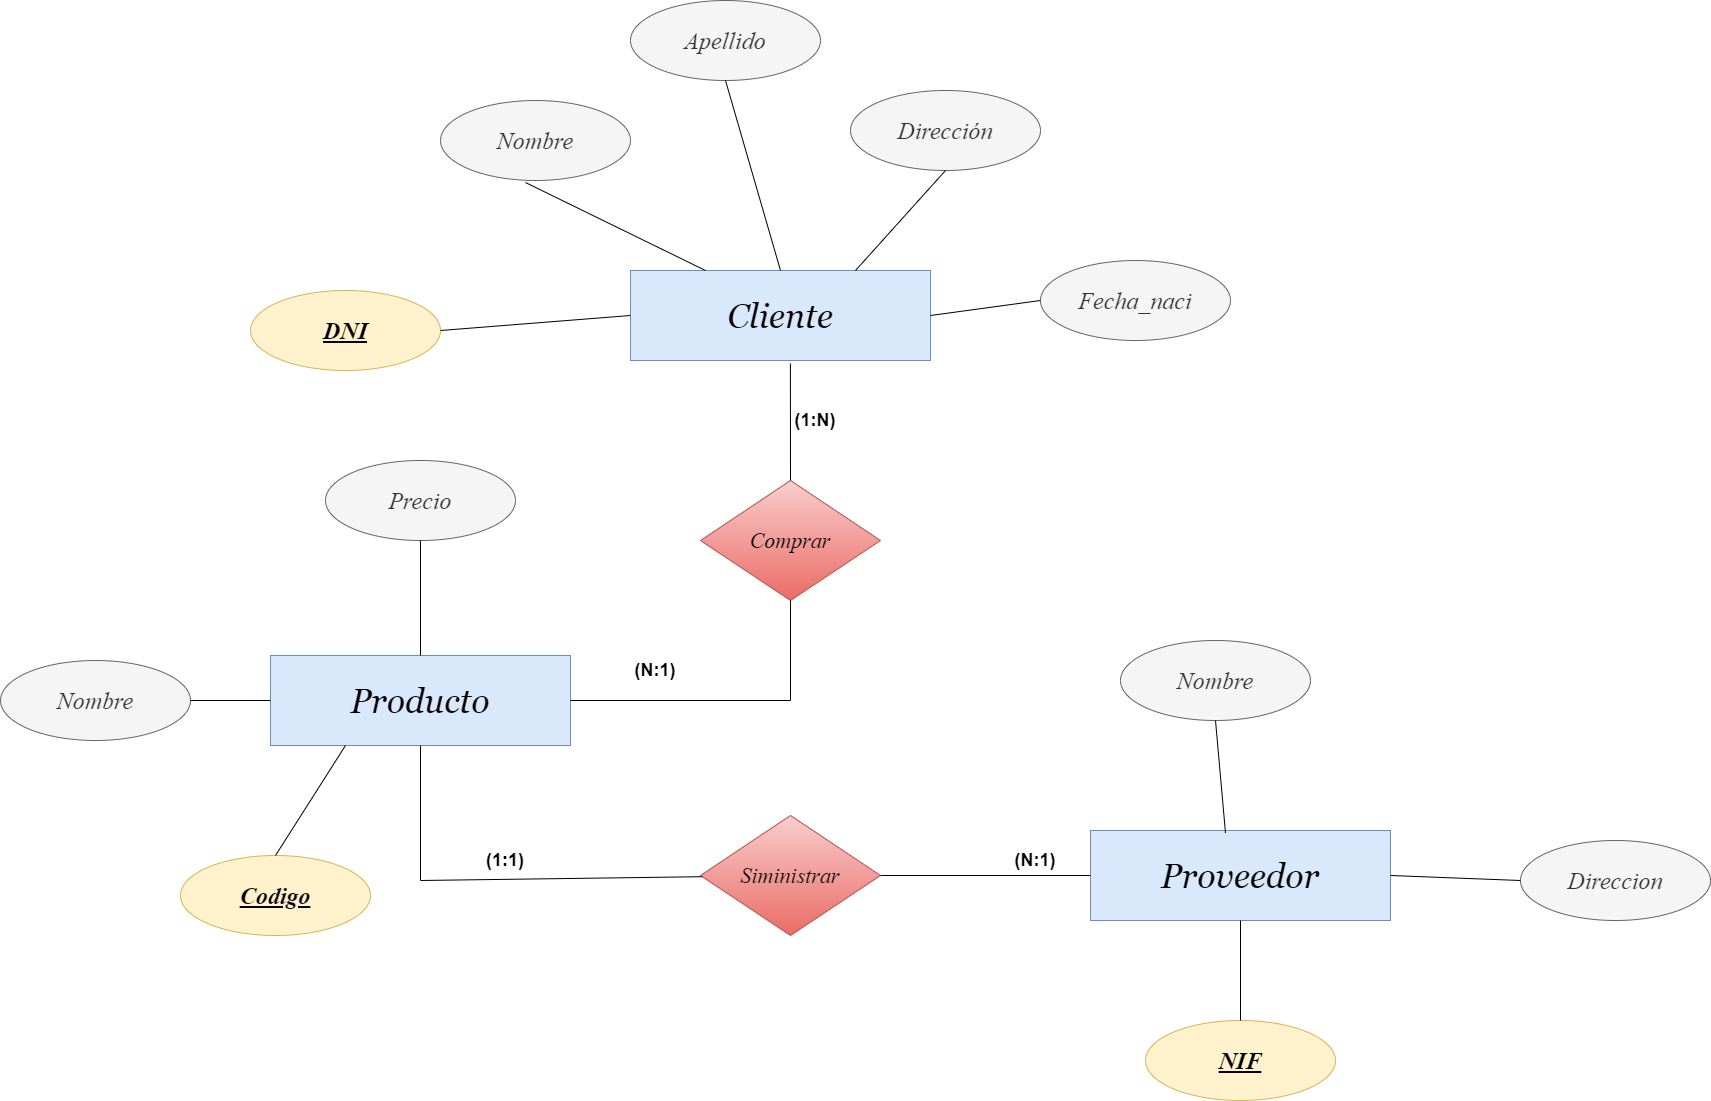
\includegraphics[width=16cm,height=10cm]{er1.png}
        \end{figure}
        \subsubsection{Diagrama Relacional}
        \begin{figure}[H]
            \centering
            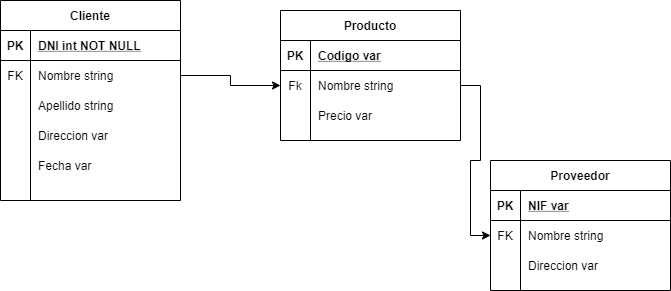
\includegraphics[width=16cm,height=10cm]{rel1.png}
        \end{figure}
        \subsubsection{Consulta de SQL}
\begin{verbatim}
CREATE DATABASE Ejercicio1_Act1;

USE Ejercicio1_Act1;

CREATE TABLE Cliente (
    DNI int primary key not null,
    Nombre varchar(50) not null,
    Apellido varchar(50) not null,
    Dirección varchar(255) not null,
    Fecha date not null
);

CREATE TABLE Producto (
    Codigo int primary key,
    Nombre varchar(100),
    Precio float not null,
    DNI int not null,
    FOREIGN KEY (DNI) REFERENCES Cliente (DNI)
);

CREATE TABLE Proveedor (
	NIF int primary key not null,
	Nombre varchar(50) not null,
	Direccion varchar(255) not null,
	Codigo int not null,
	FOREIGN KEY (Codigo) REFERENCES Producto (Codigo)
);
\end{verbatim}
        \subsubsection{Diagrama de SQL}
        \begin{figure}[H]
            \centering
            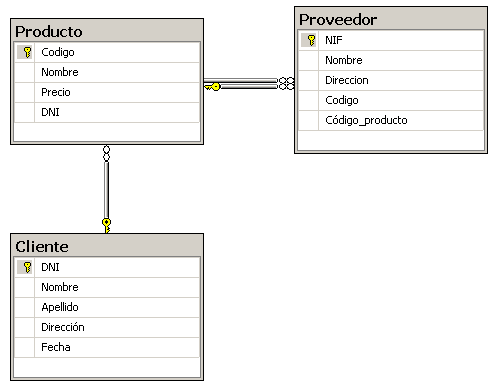
\includegraphics[width=10cm,height=10cm]{sql1.png}
        \end{figure}
        \subsubsection{Conclusión}
        \justify
        Como ya se tenia la gran mayoría de los diagramas, no hubo muchas dificultades en la implementación del ejercicio en SQL.
        \subsection{Ejercicio 2}
        \justify
        A partir del siguinte enunciado se desea realizar el modelo entidad-relación. ``Se desea informatizar la gestión de una empresa
        de transportes que reparte paquetes por toda España. Los encargados de llevar los paquetes son los camioneros, de los que se quiere
        guardar el dni, nombre, teléfono, dirección, slario y población en la que vive. De los paquetes transportados interesa conocer el
        código de paquete, descripción, destinatario y dirección del destinatario. Un camionero distribuye muchos paquetes, y un paquete sólo
        puede ser distribuido por un camionero. De las provincias a las que llegan los paquetes interesa guardar el código de provincia y el
        nombre. Un paquete sólo puede llegar a una provincia. Sin embargo, a una provincia pueden llegar varios paquetes. De los camiones que llevan
        los camioneros, interesa conocer la matrícula, modelo, tipo y potencia. Un camionero puede conducir diferentes camiones en fechas diferentes,
        y un camión puede ser conducido por varios camioneros''.
        \subsubsection{Diagrama E-R}
        \begin{figure}[H]
            \centering
            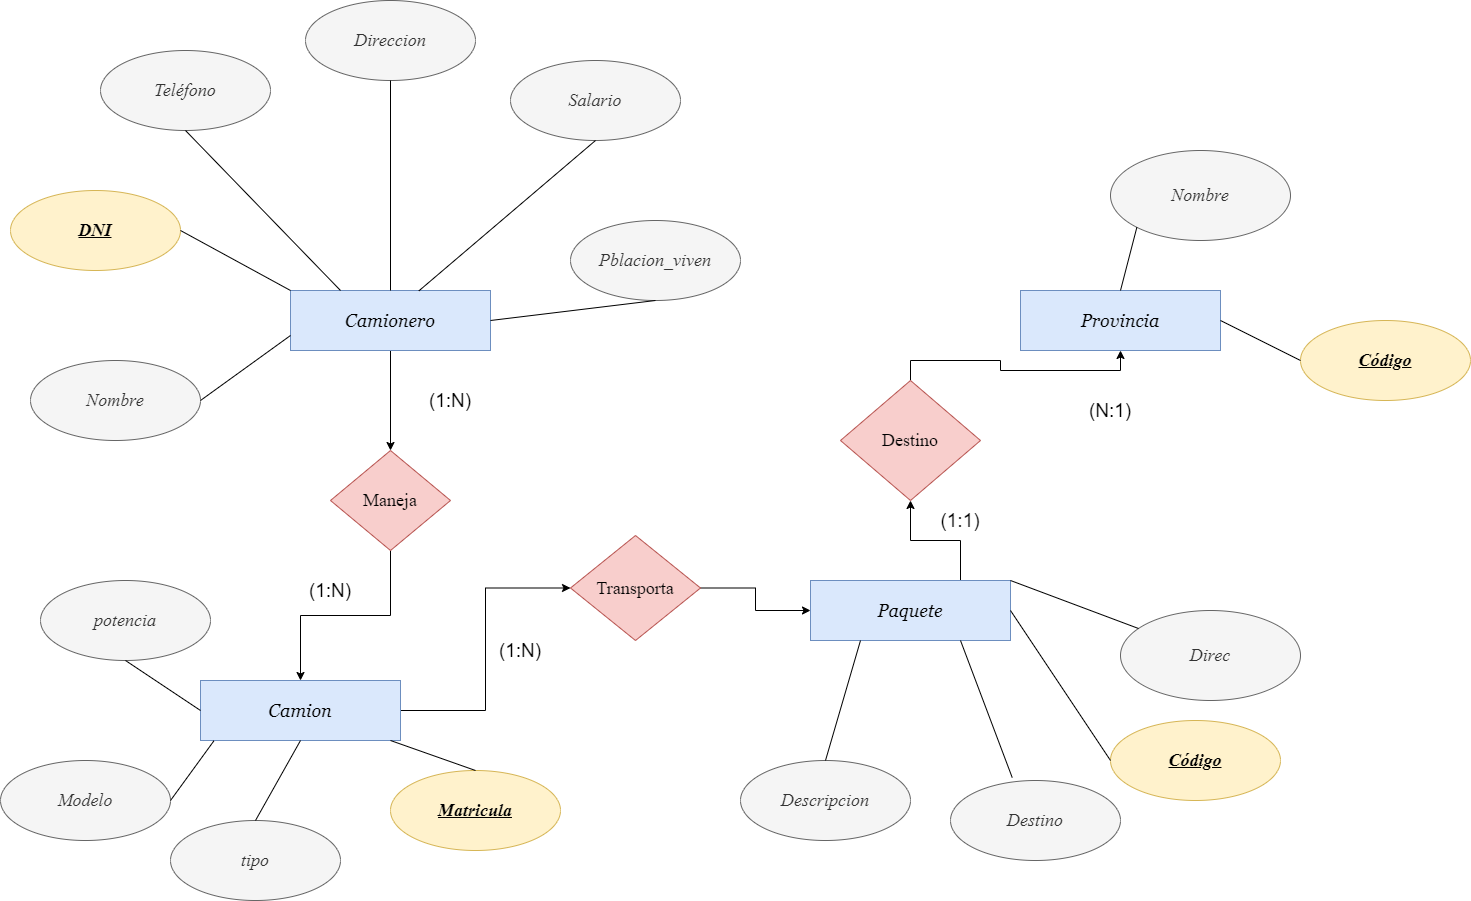
\includegraphics[width=16cm,height=10cm]{er2.png}
        \end{figure}
        \subsubsection{Diagrama Relacional}
        \begin{figure}[H]
            \centering
            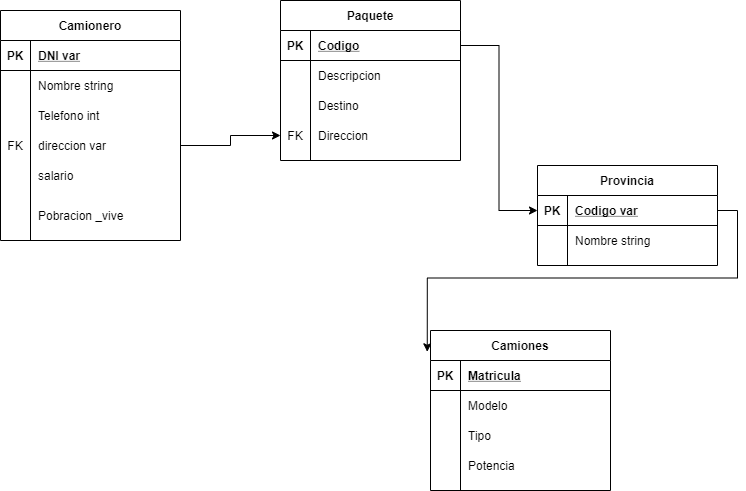
\includegraphics[width=16cm,height=10cm]{rel2.png}
        \end{figure}
        \subsubsection{Consulta de SQL}
\begin{verbatim}
CREATE DATABASE Ejercicio2_Act1;

USE Ejercicio2_Act1;

CREATE TABLE Camionero(
    DNI int primary key not null,
    Nombre varchar(50) not null,
    Telefono int not null,
    direccion varchar(255) not null,
    salario float not null,
    Población_vive varchar(50) not null
);

CREATE TABLE Paquete(
    Código int primary key not null,
    Descripcion varchar(50) not null,
    Destino varchar(255) not null,
    Dirección varchar(255) not null,
    DNI int not null,
    FOREIGN KEY (DNI) REFERENCES Camionero (DNI)
);

CREATE TABLE Provincia(
    Codigo int primary key not null,
    Nombre varchar(50) not null,
    IDPaquete int not null,
    FOREIGN KEY (IDPaquete) REFERENCES Paquete (Código)
);

CREATE TABLE Camiones(
    Matrícula int primary key not null,
    Modelo varchar(20) not null,
    Tipo varchar(20) not null,
    Potencia float not null,
    IDProvincia int not null,
    FOREIGN KEY (IDProvincia) REFERENCES Provincia (Codigo)
);
\end{verbatim}
        \subsubsection{Diagrama de SQL}
        \begin{figure}[H]
            \centering
            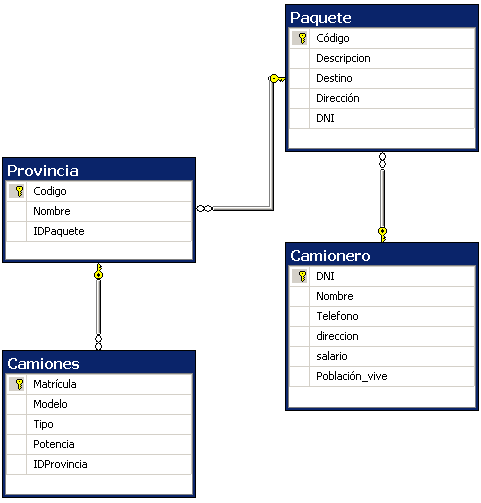
\includegraphics[width=8cm,height=10cm]{sql2.png}
        \end{figure}
        \subsubsection{Conclusión}
        \justify
        Al ser uno de los ejercicios cortos y con los diagramas hechos de antemano, no se presento mucha complicación al respecto.
        \subsection{Ejercicio 3}
        \justify
        A partir del siguiente supuesto diseñar el modelo entidad-relación. ``Se desea diseñar una base de datos para almacenar y gestionar la información
        empleada por una empresa dedicada a la venta de automóviles, teniendo en cuenta los siguientes aspectos: La empresa dispone de una serie de coches para
        su venta, Se necesita conocer la matrícula, marca y modelo; el color y el precio de venta de cada coche. Los datos que interesa conocer de cada cliente
        son el NIFm nombre, dirección, ciudad y número de teléfono: además, los clientes se diferencian por un código interno de la empresa que se incrementa
        automáticamente cuando un cliente se da de alta en ella. Un cliente puede comprar tantos coches como desee a la empresa. Un coche determinado solo puede ser comprado
        por un único cliente. El concesionario también se encarga de llevar a cabo las revisiones automáticamente por cada revisión que se haga. De cada revisión se desea saber
        si se ha hecho cambio de filtro, si se ha hecho cambio de aceite, si se ha hecho cambio de frnos u otros. Los coches pueden pasar varias revisiones en el concesionario''.
        \subsubsection{Diagrama E-R}
        \begin{figure}[H]
            \centering
            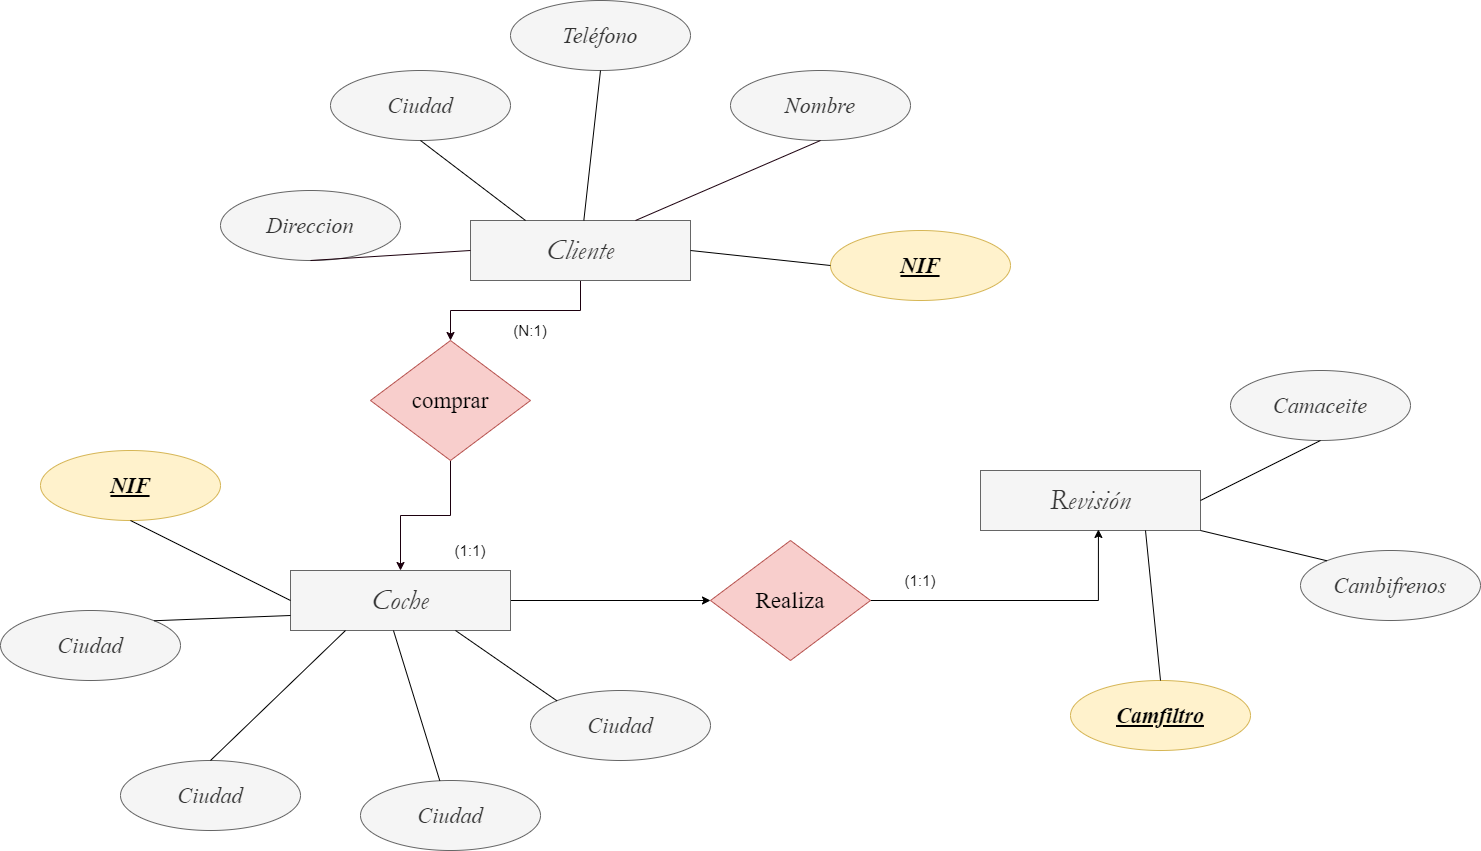
\includegraphics[width=16cm,height=10cm]{er3.png}
        \end{figure}
        \subsubsection{Diagrama Relacional}
        \begin{figure}[H]
            \centering
            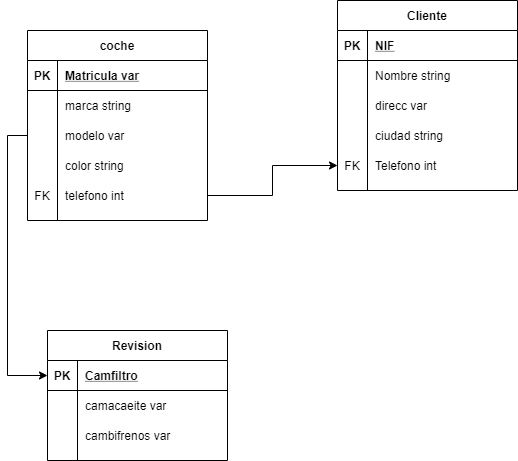
\includegraphics[width=16cm,height=10cm]{rel3.png}
        \end{figure}
        \subsubsection{Consulta de SQL}
\begin{verbatim}
CREATE DATABASE Ejercicio3_Act1;

USE Ejercicio3_Act1;

CREATE TABLE Revision(
    Camfiltro int primary key not null,
    camaceite varchar(50) not null,
    cambifrenos varchar(50) not null
);

CREATE TABLE coche(
    Matricula int primary key not null,
    marca varchar(50) not null,
    modelo varchar(20) not null,
    color varchar(20) not null,
    telefono int not null,
    Camfiltro int not null,
    FOREIGN KEY (Camfiltro) REFERENCES Revision (Camfiltro)
);

CREATE TABLE Cliente(
    NIF int primary key not null,
    Nombre varchar (50) not null,
    direcc varchar(255) not null,
    ciudad varchar(100) not null,
    Telefono int not null,
    Matricula int not null,
    FOREIGN KEY (Matricula) REFERENCES coche (Matricula)
);
\end{verbatim}
        \subsubsection{Diagrama de SQL}
        \begin{figure}[H]
            \centering
            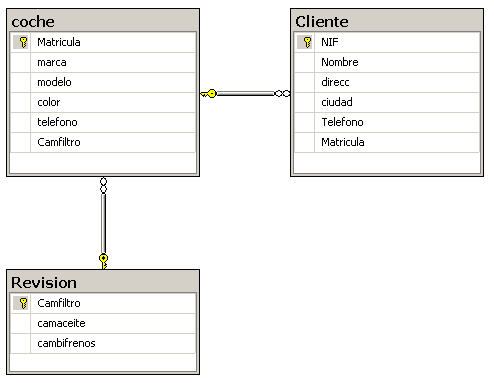
\includegraphics[width=8cm,height=8cm]{sql3.PNG}
        \end{figure}
        \subsubsection{Conclusión}
        \justify
        Similar a los anteriores, no hubo complicaciones sustanciales. Teniendo los diagramas, el planteamiento en SQL es más simple.
        \subsection{Ejercicio 4}
        \justify
        A partir del siguiente supuesto realizar el modelo entidad-relación y pasarlo a modelo relacional. ``A un concesionario de coches llegan clientes para comprar automóviles. De cada coche
        interesa saber la matrícula, modelo, marca y color. Un cliente puede comprar varios coches en el concesionario. Cuando un cliente compra un coche, se le hace una ficha en el concesionario
        con la siguiente información: dni, nombre, apellidos, dirección y teléfono. Los coches que el concesionario vende pueden ser nuevos o usados (de segunda mano). De los coches nuevos interesa
        saber el número de unidades que hay en el concesionario. De los coches viejos interesa el número de kilómetros que lleva recorridos. El concesionario también dispone de un taller en el que los
        mecánicos reparan los coches que llevan los clientes. Un mecánico repara varios coches a los largo del día, y un coche puede ser reparado por varios mecánicos. Los mecánicos tienen un dni, nombre, 
        apellidos, fecha de contratación y salario. Se desea guardar también la fecha en la que se repara cada vehículo y el número de horas que se tardó en arreglar cada automóvil''. Para el modelo entidad-
        relación resultante al modelo relacional.
        \subsubsection{Diagrama E-R}
        \begin{figure}[H]
            \centering
            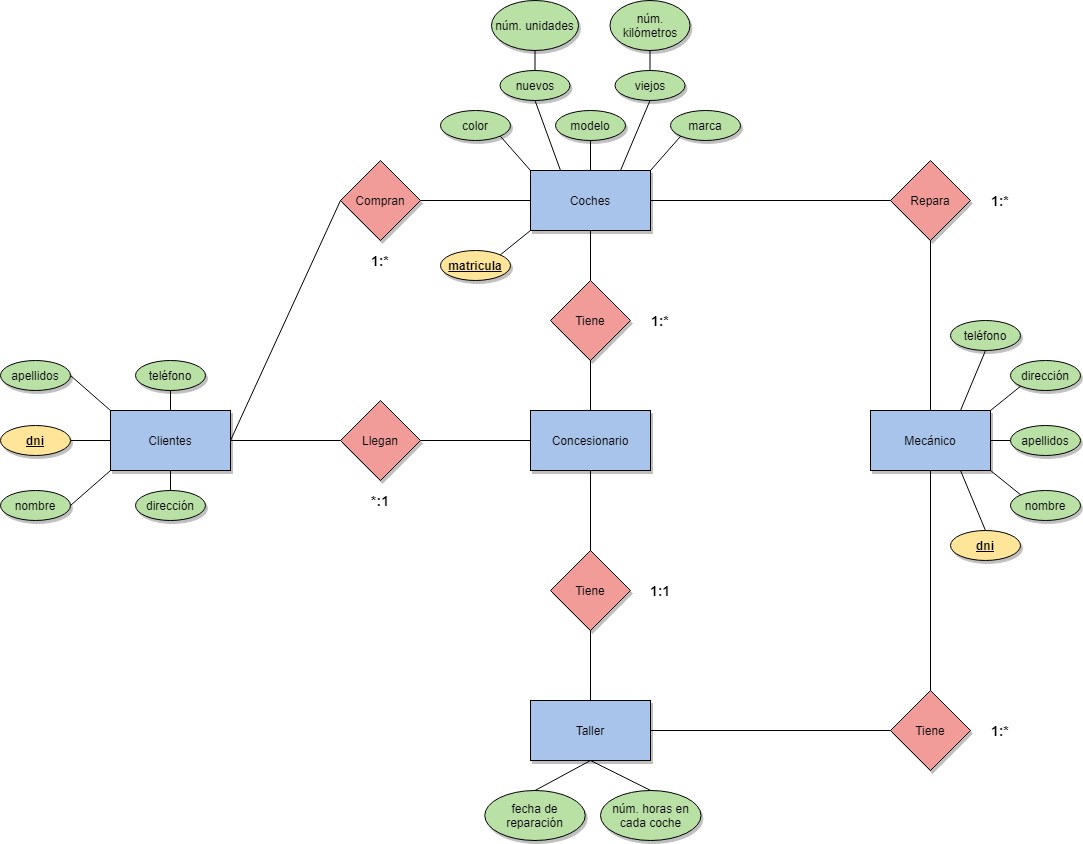
\includegraphics[width=16cm,height=10cm]{er4.png}
        \end{figure}
        \subsubsection{Diagrama Relacional}
        \begin{figure}[H]
            \centering
            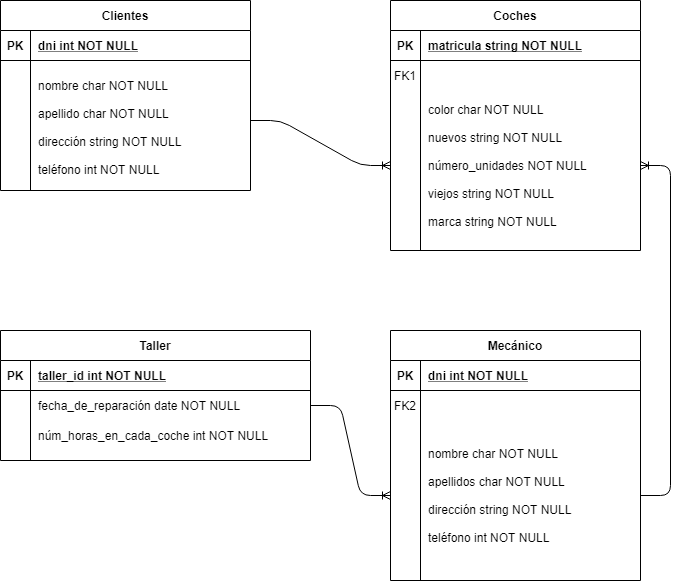
\includegraphics[width=16cm,height=6cm]{rel4.png}
        \end{figure}
        \subsubsection{Consulta de SQL}
\begin{verbatim}
CREATE DATABASE Ejercicio4_Act1;

USE Ejercicio4_Act1;

CREATE TABLE Clientes(
    dni int primary key not null,
    nombre varchar(50) not null,
    dirección varchar(255) not null,
    teléfono int not null
);

CREATE TABLE Taller(
    taller_id int primary key not null,
    fecha_de_reparación date not null,
    núm_horas_en_cada_coche int not null
);

CREATE TABLE Mecánico(
    dni int primary key not null,
    nombre varchar(50) not null,
    apellidos varchar(50) not null,
    dirección varchar(255) not null,
    teléfono int not null,
    taller_id int not null,
    FOREIGN KEY (taller_id) REFERENCES Taller (taller_id)
);

CREATE TABLE  Coches(
    matricula varchar primary key not null,
    color varchar(20) not null,
    nuevos varchar(2) not null,
    viejos varchar(2) not null,
    número_unidades int not null,
    marca varchar(10) not null,
    id_cliente int not null,
    id_mecánico int not null,
    FOREIGN KEY (id_cliente) REFERENCES Clientes (dni),
    FOREIGN KEY (id_mecánico) REFERENCES Mecánico (dni)
);
\end{verbatim}
        \subsubsection{Diagrama de SQL}
        \begin{figure}[H]
            \centering
            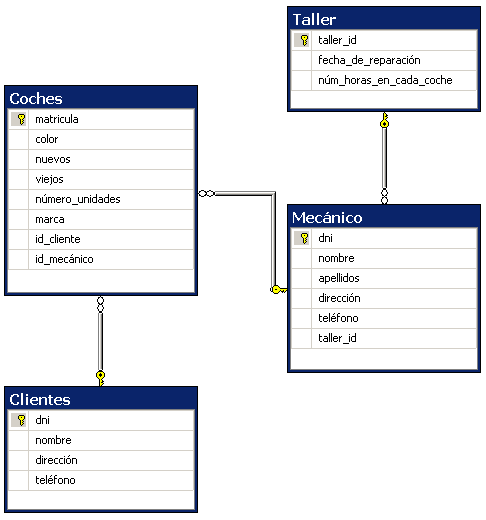
\includegraphics[width=10cm,height=10cm]{sql4.png}
        \end{figure}
        \subsubsection{Conclusión}
        \justify
        Este es uno de los ejercicios complicados debido a tener los diagramas más elaborados. Por ende se presentó dificultades para organizar todo en SQL.
        \subsection{Ejercicio 5}
        \justify
        La liga de fútbol profesional, presidida por Janito Rodríguez, ha decidido informatizar sus instalaciones creando una base de datos para guardar la información de los partidos que se juegan en la liga.
        Se desea guardar en primer lugar los datos de los jugadores. De cada jugador se quiere guardar el nombre, fecha de nacimiento y posición en la que juega (portero, defensa, centrocampísta...). Cada jugador
        tiene un código de jugador que lo identifica de manera única. De cada uno de los equipos de la liga es necesario registrar el nombre del equipo, nombre del estadio en el que juega, el aforo que tiene, el año
        de fundación del equipo y la ciudad de la que es el equipo. Cada equipo también tiene un código que lo identifica de manera única. Un jugador solo puede pertenecer a un único equipo. De cada partido que los equipos
        de la liga juegan hay que registrar la fecha en la que se juega el partido, los goles que ha metido el equipo de casa y los goles que ha metido el equipo de fuera. Cada partido tendrá un código numérico para identificar
        el partido. También se quiere llevar un recuento de los goles que hay en cada partido. Se quiere almacenar el minuto en el que se realiza el gol y la descripción del gol. Un partido tiene varios goles y un jugador
        puede meter varios goles en un partido. Por último se quiere almacenar, en la base de datos, los datos de los presidentes de los equipos de fútbol (dni, nombre, apellidos, fecha de nacimiento, equipo del que es presidente
        y año en el que fue elegido presidente). Un equipo de fútbol tan sólo puede tener un presidente, y una persona sólo puede ser presidente de un equipo de la liga. Parar el modelo entidad-relación resultante al modelo relacional.
        \subsubsection{Diagrama E-R}
        \begin{figure}[H]
            \centering
            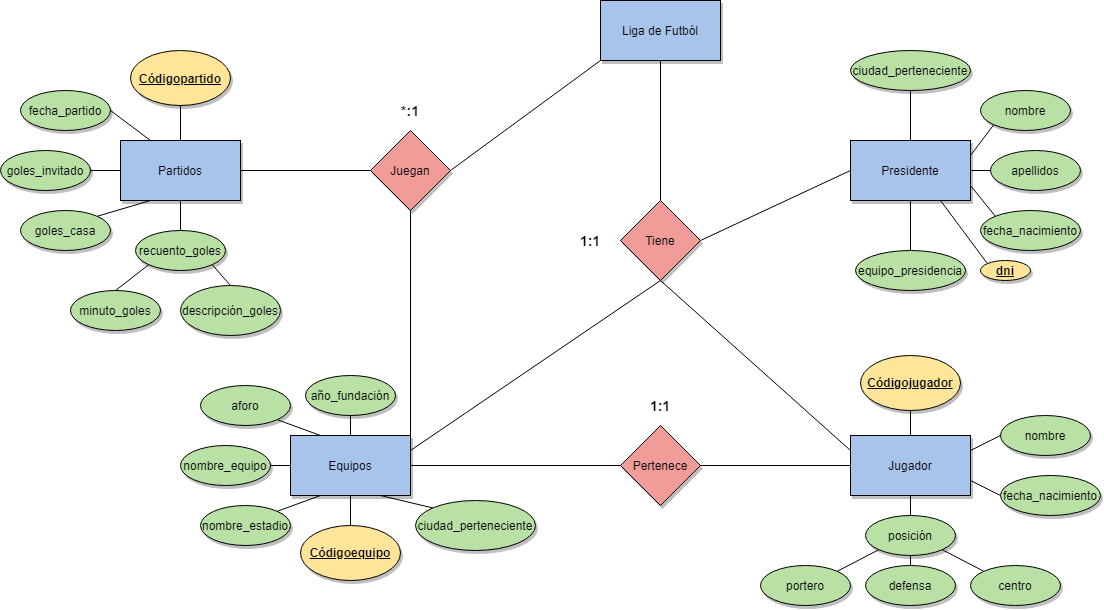
\includegraphics[width=16cm,height=10cm]{er5.png}
        \end{figure}
        \subsubsection{Diagrama Relacional}
        \begin{figure}[H]
            \centering
            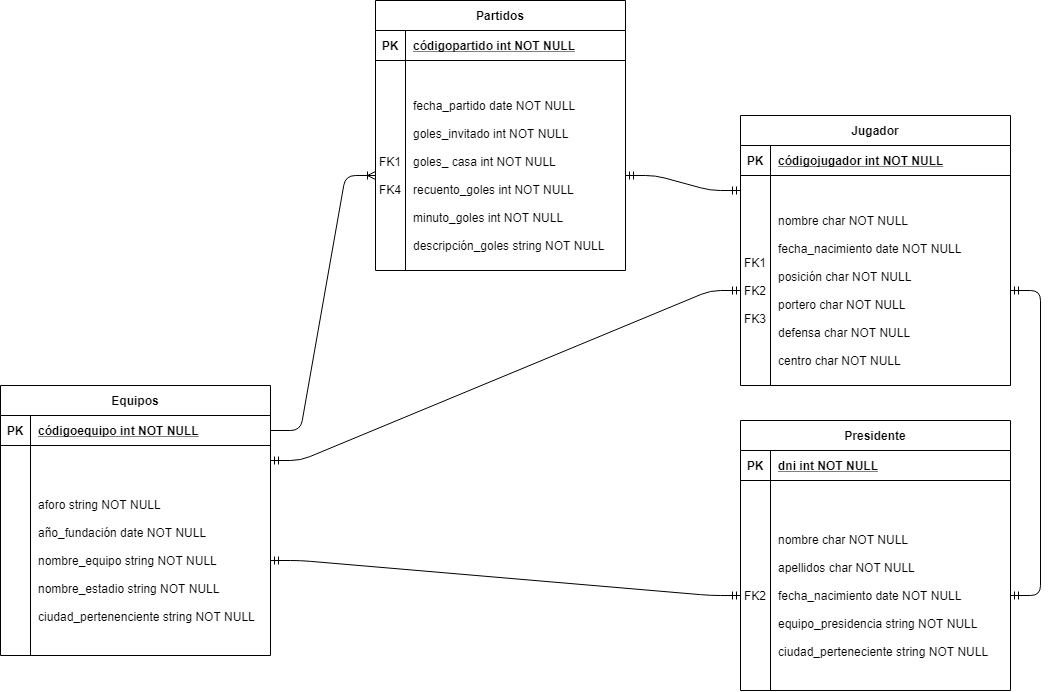
\includegraphics[width=16cm,height=10cm]{rel5.png}
        \end{figure}
        \subsubsection{Consulta de SQL}
\begin{verbatim}
CREATE DATABASE Ejercicio5_Act1;

USE Ejercicio5_Act1;

CREATE TABLE Equipos(
    códigoequipo int primary key not null,
    aforo varchar(50) not null,
    año_fundación date not null,
    nombre_equipo varchar not null,
    nombre_estadio varchar not null,
    ciudad_perteneciente varchar not null
);

CREATE TABLE Presidente(
    dni int primary key not null,
    nombre varchar(50) not null,
    apellidos varchar(50) not null,
    fecha_nacimiento date not null,
    equipo_presidencia varchar not null,
    ciudad_perteneciente varchar not null,
    códigoequipo int not null,
    FOREIGN KEY (códigoequipo) REFERENCES Equipos (códigoequipo)
);

CREATE TABLE Partidos(
	códigopartido int primary key not null,
    fecha_partido date not null,
    goles_invitado int not null,
    goles_casa int not null,
    recuento_goles int not null,
    minuto_goles int not null,
    descripción_goles varchar not null,
    códigoequipo int not null,
    FOREIGN KEY (códigoequipo) REFERENCES Equipos (códigoequipo)
);

CREATE TABLE Jugador(
    códigojugador int primary key not null,
    nombre varchar(50) not null,
    fecha_nacimiento date not null,
    posición varchar(50) not null,
    portero varchar(2) not null,
    defensa varchar(2) not null,
    centro varchar(2) not null,
    códigoequipo int not null,
    códigopartido int not null,
    dni_presidente int not null,
    FOREIGN KEY (códigoequipo) REFERENCES Equipos (códigoequipo),
    FOREIGN KEY (códigopartido) REFERENCES Partidos (códigopartido),
    FOREIGN KEY (dni_presidente) REFERENCES Presidente (dni)
);
\end{verbatim}
        \subsubsection{Diagrama de SQL}
        \begin{figure}[H]
            \centering
            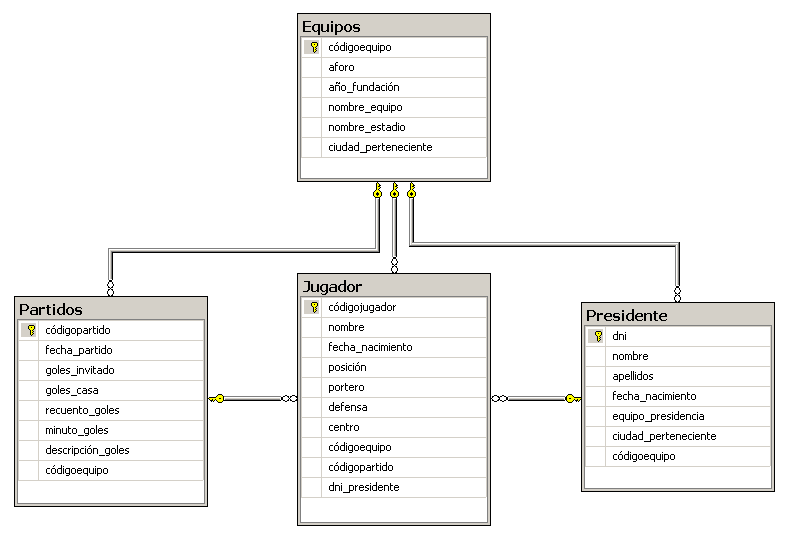
\includegraphics[width=12cm,height=12cm]{sql5.png}
        \end{figure}
        \subsubsection{Conclusión}
        \justify
        A pesar de tener el diagrama relación extenso, su implementación a SQL es bastante sencilla. Como en ejercicios anteriores, no existen muchas complicaciones mas allá de los errores de redacción.
        \subsection{Ejercicio 6}
        \justify
        Una agencia de viajes desea informatizar toda la gestión de los viajeros que acuden a la agencia y los viajes que estos realizan. Tras ponernos en contacto con la agencia, ésta nos proporciona la siguiente información. ``La agencia 
        desea guardar la siguiente información de los viajeros: dni, nombre, dirección y teléfono. De cada uno de los viajes que maneja la agencia interesa guardar el código de viaje, número de plazas, fecha en la que se realiza el viaje y
        otros datos. Un viajero puede realizar tantos viajes como desee con la agencia, Un viaje determinado sólo puede ser cubierto por un viajero. Cada viaje realizado tiene un destino y un lugar de origen. De cada uno de ellos se quiere almacenar
        el código, nombre y otros datos que puedan ser de interés. Un viaje tiene un único lugar de destino y un único lugar de origen''. Realizar el modelo E-R.
        \subsubsection{Diagrama E-R}
        \begin{figure}[H]
            \centering
            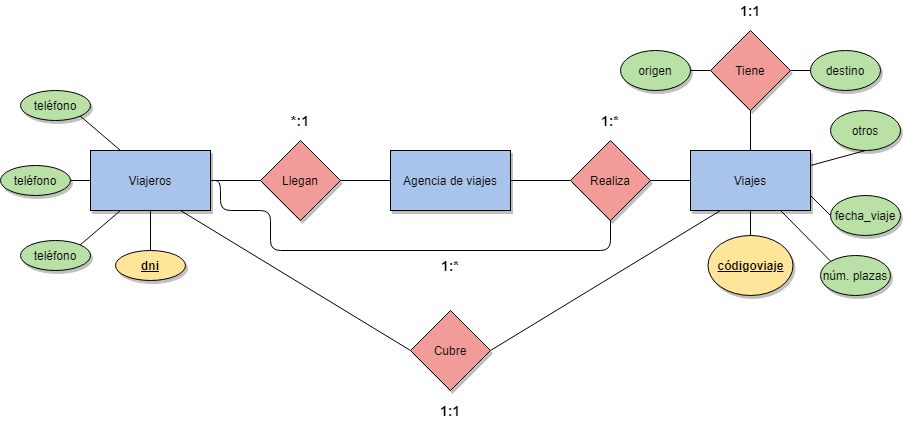
\includegraphics[width=16cm,height=10cm]{er6.png}
        \end{figure}
        \subsubsection{Diagrama Relacional}
        \begin{figure}[H]
            \centering
            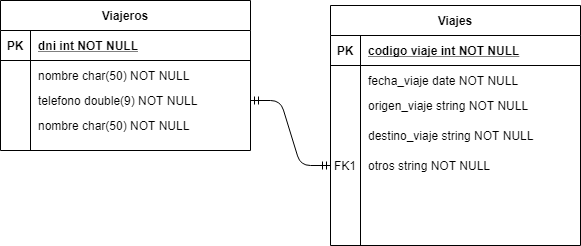
\includegraphics[width=16cm,height=10cm]{rel6.png}
        \end{figure}
        \subsubsection{Consulta de SQL}
\begin{verbatim}
CREATE DATABASE Ejercicio6_Act1;

USE Ejercicio6_Act1;

CREATE TABLE Viajeros(
    dni int primary key not null,
    nombre varchar(50) not null,
    telefono int not null,
);

CREATE TABLE Viajes(
    código_viaje int primary key not null,
    fecha_viaje date not null,
    origen_viaje varchar not null,
    destino_viaje varchar not null,
    otros varchar not null,
    dni int not null,
    FOREIGN KEY (dni) REFERENCES Viajeros (dni)
);
\end{verbatim}
        \subsubsection{Diagrama de SQL}
        \begin{figure}[H]
            \centering
            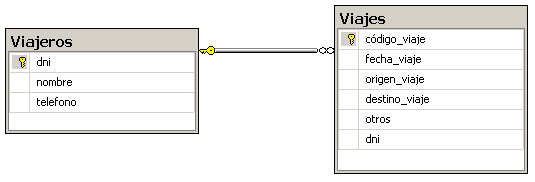
\includegraphics[width=12cm,height=8cm]{sql6.PNG}
        \end{figure}
        \subsubsection{Conclusión}
        \justify
        Este fue el ejercicio más sencillo de todos. Debido a que su diagrama E-R solo contiene dos relaciones, la implementación en SQL fue muy simple.
        \subsection{Ejercicio 7}
        \justify
        Se quiere modelar la realidad relativa a una clínica odontológica.
        \subsubsection{Diagrama E-R}
        \begin{figure}[H]
            \centering
            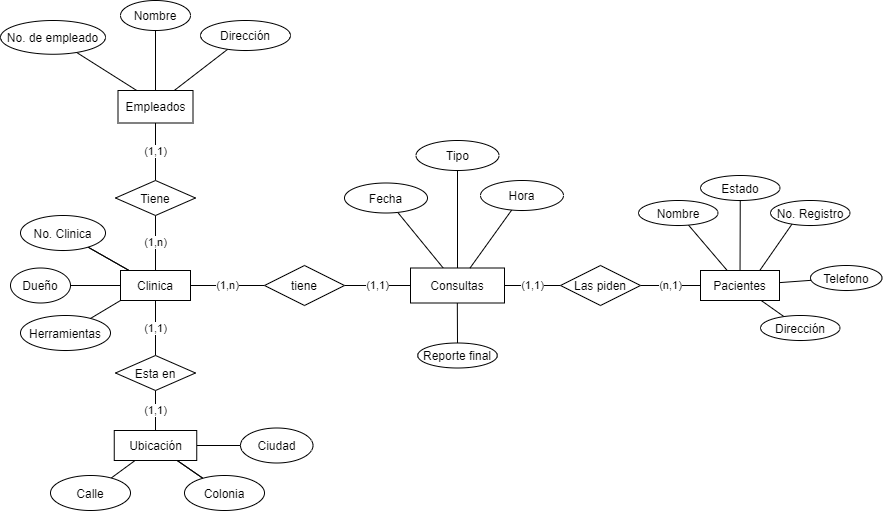
\includegraphics[width=16cm,height=10cm]{er7.png}
        \end{figure}
        \subsubsection{Diagrama Relacional}
        \begin{figure}[H]
            \centering
            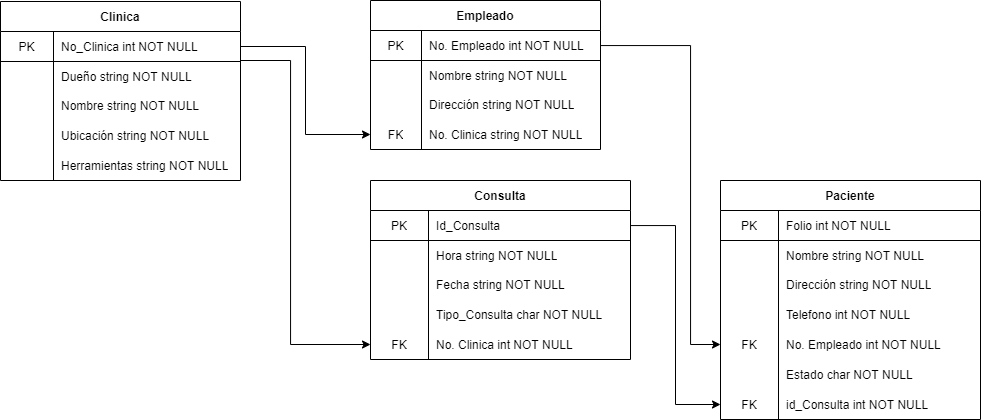
\includegraphics[width=16cm,height=10cm]{rel7.png}
        \end{figure}
        \subsubsection{Consulta de SQL}
\begin{verbatim}
CREATE DATABASE Ejercicio7_Act1;

USE Ejercicio7_Act1;

CREATE TABLE Clinica(
    No_Clinica int primary key not null,
    Dueño varchar not null,
    Nombre varchar not null,
    Ubicación varchar not null,
    Herramientas varchar not null
);

CREATE TABLE Empleado(
    No_Empleado int primary key not null,
    Nombre varchar not null,
    Dirección varchar not null,
    No_Clínica int not null,
    FOREIGN KEY (No_Clínica) REFERENCES Clinica (No_Clinica)
);

CREATE TABLE Consulta(
    id_Consulta int primary key not null,
    Hora varchar not null,
    Fecha varchar not null,
    Tipo_Consulta varchar(50) not null,
    No_Clínica int not null,
    FOREIGN KEY (No_Clínica) REFERENCES Clinica (No_Clinica)
);

CREATE TABLE Paciente(
    Folio int primary key not null,
    Nombre varchar not null,
    Dirección varchar not null,
    Telefono int not null,
    Estado varchar(50) not null,
    No_Empleado int not null,
    id_Consulta int not null,
    FOREIGN KEY (No_Empleado) REFERENCES Empleado (No_Empleado),
    FOREIGN KEY (id_Consulta) REFERENCES Consulta (id_COnsulta)
);
\end{verbatim}
        \subsubsection{Diagrama de SQL}
        \begin{figure}[H]
            \centering
            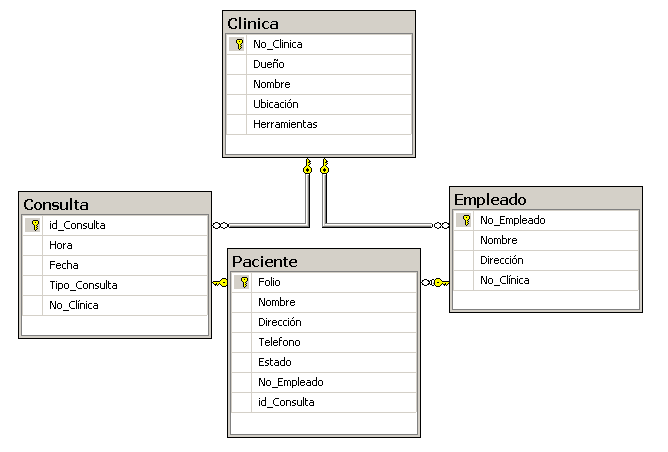
\includegraphics[width=12cm,height=10cm]{sql7.PNG}
        \end{figure}
        \subsubsection{Conclusión}
        \justify
        En lo que cabe de su creación, como solo se provió de una instrucción muy vaga, se vió en la necesidad de improvisar los posibles diagramas relacional y E-R para aplicar el resto de implementaciones.
        \subsection{Ejercicio 8}
        \justify
        Las sedes olímpicas se dividen en complejos deportivos. Los complejos deportivos se subdividen en aquellos en los que se desarrolla un único deporte y en los polideportivos. Los complejos polideportivos tienen áreas designadas para cada deporte
        con un indicador de localización (ejemplo: centro, esquinaNE, etc.). Un complejo tiene una localización, un jefe de organización individual y un área total ocupada. Los dos tipos de complejos (deporte único y polideportivo) tendrán diferentes tipos de información.
        Para cada tipo de sesde, se conservará el número de complejos junto con su presupuesto aproximado. Cada complejo celebra una serie de eventos (ejemplo: la pista del estadio puede celebrar muchar carreras distintas). Para cada evento está prevista una fecha,
        duración, número de participantes, número de comisarios. Una lista de todos los comisarios se conservará junto con la lista de los eventos en los que esté involucrado cada comisario ya sea cumpliendo la tarea de juez u observador. Tanto para cada evento como para el
        manteniemiento se necesitará cierto equipamiento (ejemplo: arcos, pértigas, barras paralelas, etc.).
        \subsubsection{Diagrama E-R}
        \begin{figure}[H]
            \centering
            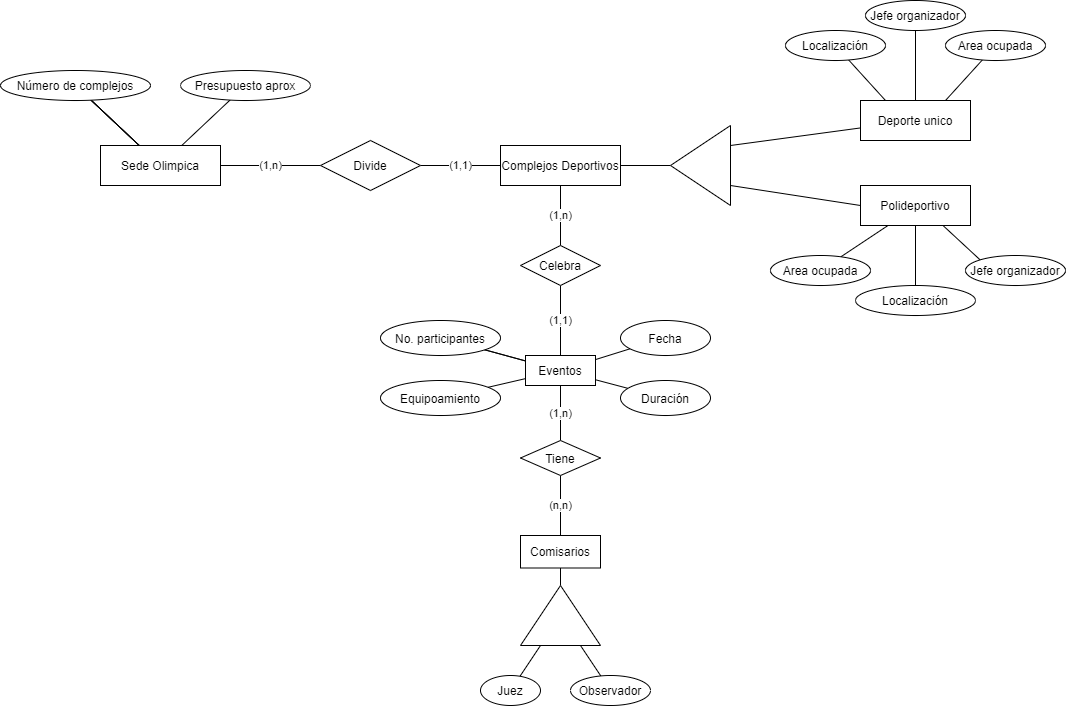
\includegraphics[width=16cm,height=10cm]{er8.png}
        \end{figure}
        \subsubsection{Diagrama Relacional}
        \begin{figure}[H]
            \centering
            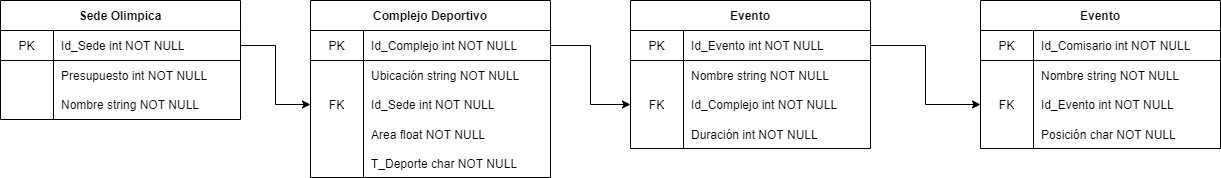
\includegraphics[width=15cm,height=7cm]{rel8.jpg}
        \end{figure}
        \subsubsection{Consulta de SQL}
\begin{verbatim}
CREATE DATABASE Ejercicio8_Act1;

USE Ejercicio8_Act1;

CREATE TABLE Sede_Olimpica(
    Id_Sede int primary key not null,
    Presupuesto int not null,
    Nombre varchar not null
);

CREATE TABLE Complejo_Deportivo(
    Id_Complejo int primary key not null,
    Ubicación varchar not null,
    Area float not null,
    T_Deporte varchar(50) not null,
    Id_Sede int not null,
    FOREIGN KEY (Id_Sede) REFERENCES Sede_Olimpica (Id_Sede)
);

CREATE TABLE Evento(
    Id_Evento int primary key not null,
    Nombre varchar not null,
    Duración int not null,
    Id_Complejo int not null,
    FOREIGN KEY (Id_Complejo) REFERENCES Complejo_Deportivo (Id_Complejo)
);

CREATE TABLE Encargado_Evento(
    Id_Comisario int primary key not null,
    Nombre varchar not null,
    Posición varchar(50) not null,
    Id_Evento int not null,
    FOREIGN KEY (Id_Evento) REFERENCES Evento (Id_Evento)
);
\end{verbatim}
        \subsubsection{Diagrama de SQL}
        \begin{figure}[H]
            \centering
            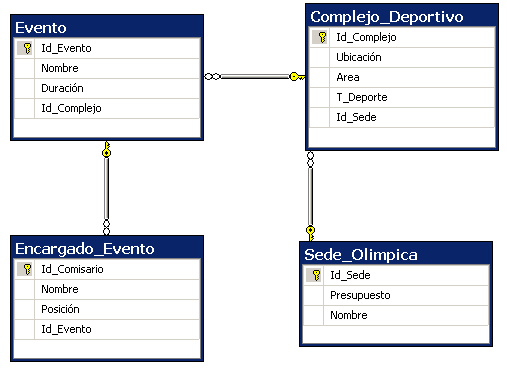
\includegraphics[width=10cm,height=10cm]{sql8.PNG}
        \end{figure}
        \subsubsection{Conclusión}
        \justify
        Similar a los ejercicios anteriores, su implementación no causo problema ya que solo se presentó una llave primaria por cada relación.
        \subsection{Ejercicio 9}
        \justify
        El sistema debe memorizar todos los encuentros que se han desarrollado desde que existe el torneo, así como las siguientes características de estos.\\
        \textbf{Descripción:} El Grand Slam se compone de cuatro torneas anuales que se celebran en Gran Bretaña, Estados Unidos, Francia y Australia. En cada país se pueden desarrollar en distintos lugares
        (p- ej., en EE.UU. puede desarrikkarse eb Forest Hill o en Flashing Meadows). Cada partido tiene asociado un premio de consolación para el perdedor que dependerá de la fase en que se encuentre el torneo (p. ej., el perdedor octavos de final puede ganar 5,000 dólares).
        El ganador de la final recibirá el premio correspondiente al torneo. Cada torneo tiene cienco modalidades: Indivual masculino, individual femenino, dobles masculino, dobles femenino y dobles mixtos. También hay que tener en cuenta la nacionalidad de un jugador, de forma que
        este puede ser apátrida o tener varias nacionalidades.\\
        \textbf{Resultados a considerar:} El sistema debe dar respuesta a las siguentes preguntas:
        \begin{enumerate}
            \item Dado un año y un torneo, composición y resultado de los partidos.
            \item Lista de árbitros que participaron en el torneo.
            \item Ganancias percibidas en premios por un jugador a lo largo del torneo.
            \item Lista de entrenadores que han entrenado a un jugador a lo largo del torneo y fechas en las que lo hizo.
        \end{enumerate} 
        Ejemplos de acceso a la base de datos:
        \begin{enumerate}
            \item Connors ganó Gerulaitis en Roland Garros en 1979 en cuartos de final en individuales masculinos por 6-3 4-3/7-5 6-0.
            \item El señor Wlkinson árbitro ese partido.
            \item Alemanio ha ganado dos veces las individuales masculinas de Wimbledon. Borg ha ganado 2,000,000 de dólares a lo largo de su participación en el Grand Slam.
            \item El ganador de Roland Garros de 1987 ganó 20,000 dólares.
            \item Noah ha jugado cuatro veces en dobles mixtos con Mandlikova.
        \end{enumerate}
        \subsubsection{Diagrama E-R}
        \begin{figure}[H]
            \centering
            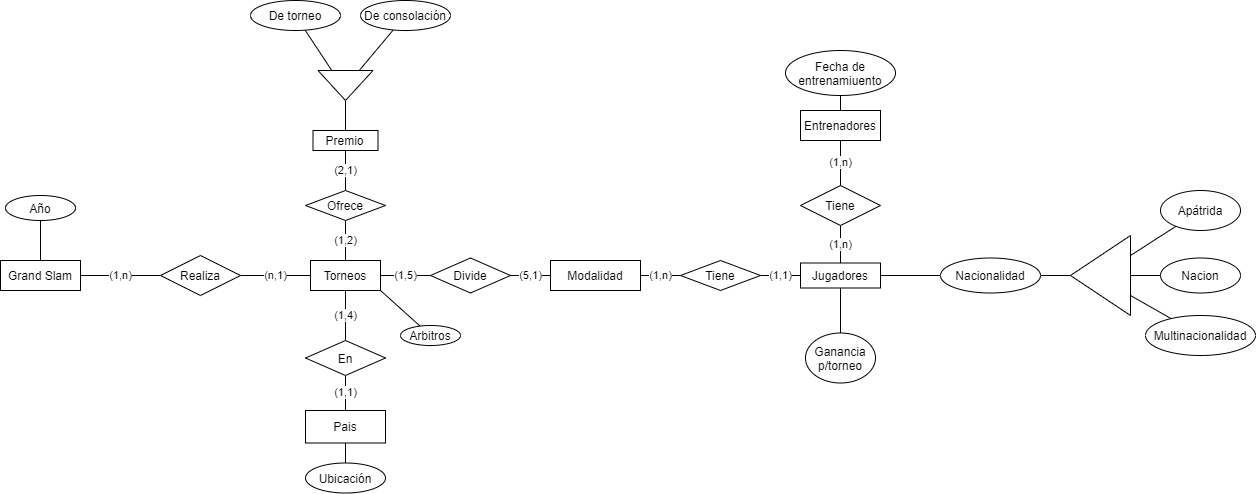
\includegraphics[width=16cm,height=10cm]{er9.png}
        \end{figure}
        \subsubsection{Diagrama Relacional}
        \begin{figure}[H]
            \centering
            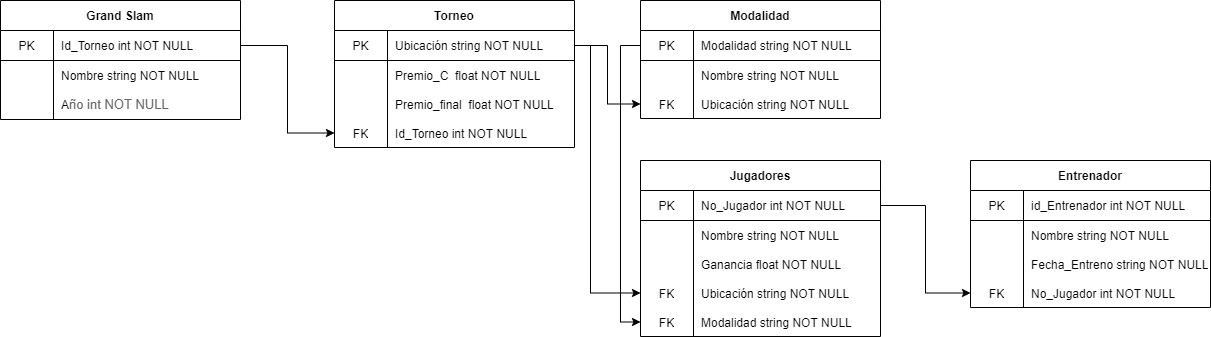
\includegraphics[width=16cm,height=10cm]{rel9.jpg}
        \end{figure}
        \subsubsection{Consulta de SQL}
\begin{verbatim}
CREATE DATABASE Ejercicio9_Act1;

USE Ejercicio9_Act1;

CREATE TABLE Grand_Slam(
    Id_Torneo int primary key not null,
    Nombre string not null,
    Año int not null
);

CREATE TABLE Torneo(
    Ubicación string primary key not null,
    Premio_C float not null,
    Premio_final float not null,
    Id_Torneo int not nullm
    FOREIGN KEY (Id_Torneo) REFERENCES Grand_Slam (Id_Torneo)
);

CREATE TABLE Modalidad(
    Modalidad string primary key not null,
    Nombre string not null,
    Ubicación string not null,
    FOREIGN KEY (Ubicación) REFERENCES Torneo (Ubicación)
);

CREATE TABLE Jugadores(
    No_Jugador int not null,
    Nombre string not null,
    Ganancia float not null,
    Ubicación string not null,
    Modalidad string not null,
    FOREIGN KEY (Ubicación) REFERENCES Torneo (Ubicación),
    FOREIGN KEY (Modalidad) REFERENCES Modalidad (Modalidad)
);

CREATE TABLE Entrenado(
    id_Entrenador int primary key not null,
    Nombre string not null,
    Fecha_Entreno string not null,
    No_Jugador int not null,
    FOREIGN KEY (No_Jugador) REFERENCES Jugadores (No_Jugador)
);
\end{verbatim}
        \subsubsection{Diagrama de SQL}
        \begin{figure}[H]
            \centering
            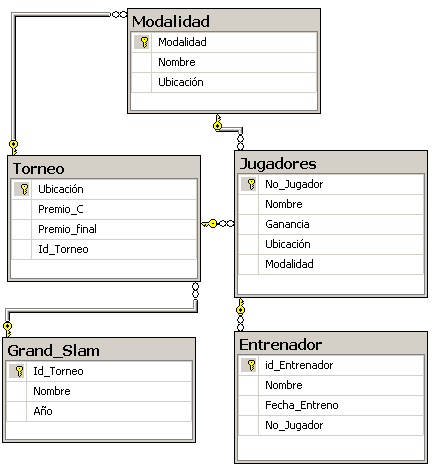
\includegraphics[width=10cm,height=10cm]{sql9.PNG}
        \end{figure}
        \subsubsection{Conclusión}
        \justify
        Fue uno de los diagramas más complejos a implementar debido a tener muchas llaves primarias, lo que la mala implementación de las mismas causa estragos en la ejecución de las consultas de SQL.
        \section{Actividad: U3T2 Conversión E-R a Relacional}
        \subsection{Ejercicio 1}
        \justify
        A partir del siguiente enunciado se desea realizar el modelo entidad-relación.
        ``Una empresa vende productos a varios clientes. Se necesita conocer los datos personales de los clientes
        (nombre, apellidos dni, dirección y fecha de nacimiento). Cada producto tiene un nombre y un código, así como un precio
        unitario. Un cliente puede comprar varios clientes. Los productos son suministrados por diferentes proveedores.
        Se debe tener en cuenta que un producto sólo puede ser suministrado por un proveedor, y que un proveedor puede
        suministrar diferentes productos. De cada proveedor se desea conocer el NIF, nombre y dirección.''
        \subsubsection{Diagrama E-R}
        \begin{figure}[H]
            \centering
            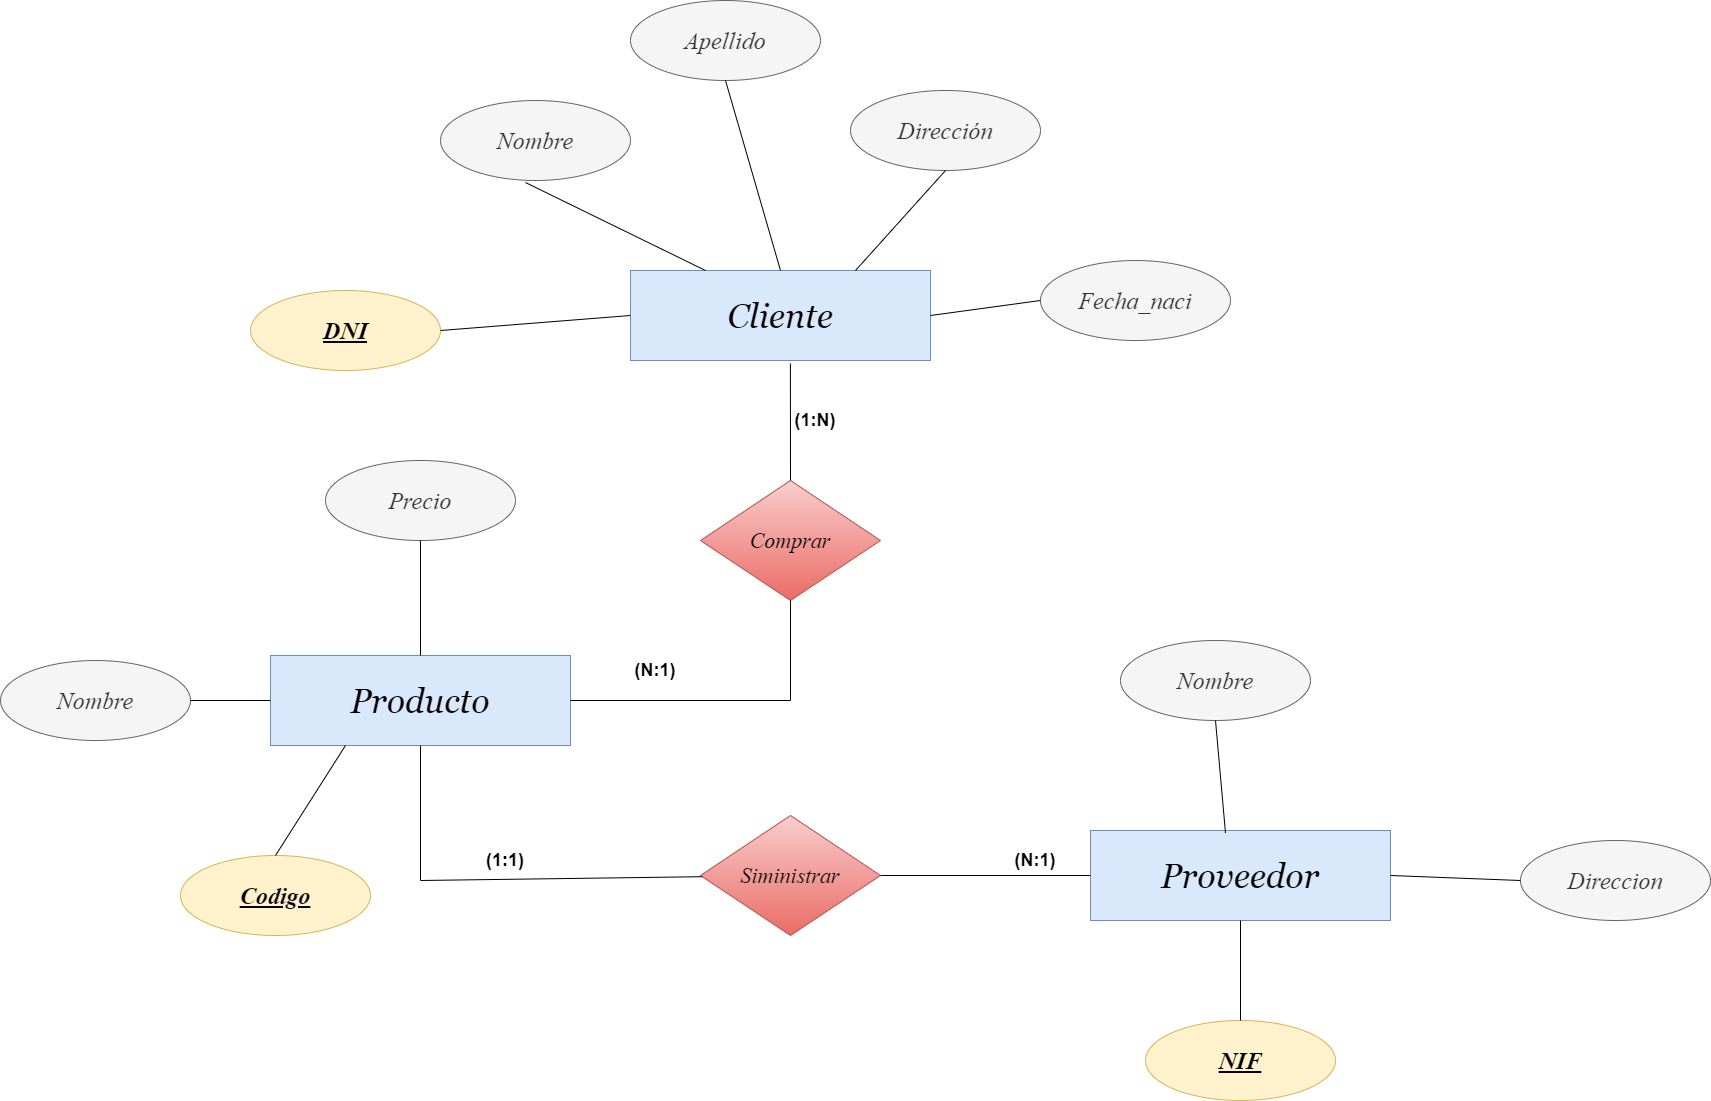
\includegraphics[width=16cm,height=10cm]{er1.png}
        \end{figure}
        \subsubsection{Diagrama Relacional}
        \begin{figure}[H]
            \centering
            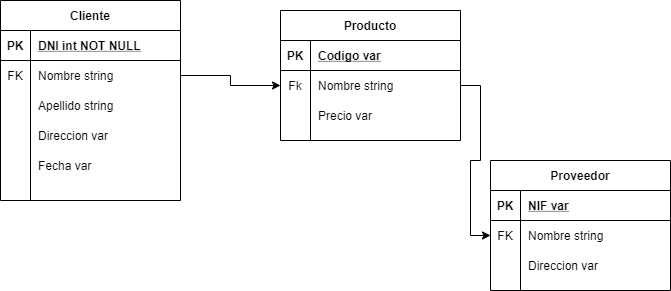
\includegraphics[width=16cm,height=10cm]{rel1.png}
        \end{figure}
        \subsubsection{Consulta de SQL}
\begin{verbatim}
CREATE DATABASE Ejercicio1_Act1;

USE Ejercicio1_Act1;

CREATE TABLE Cliente (
    DNI int primary key not null,
    Nombre varchar(50) not null,
    Apellido varchar(50) not null,
    Dirección varchar(255) not null,
    Fecha date not null
);

CREATE TABLE Producto (
    Codigo int primary key,
    Nombre varchar(100),
    Precio float not null,
    DNI int not null,
    FOREIGN KEY (DNI) REFERENCES Cliente (DNI)
);

CREATE TABLE Proveedor (
	NIF int primary key not null,
	Nombre varchar(50) not null,
	Direccion varchar(255) not null,
	Codigo int not null,
	FOREIGN KEY (Codigo) REFERENCES Producto (Codigo)
);
\end{verbatim}
        \subsubsection{Diagrama de SQL}
        \begin{figure}[H]
            \centering
            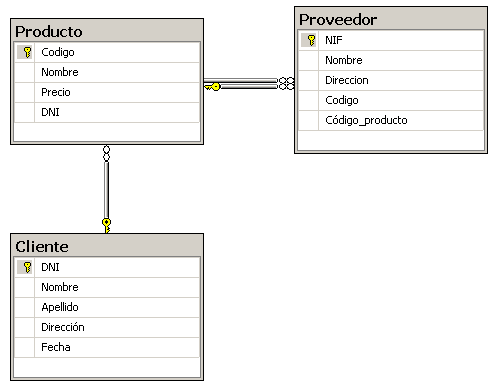
\includegraphics[width=10cm,height=10cm]{sql1.png}
        \end{figure}
        \subsubsection{Conclusión}
        \justify
        Como ya se tenia la gran mayoría de los diagramas, no hubo muchas dificultades en la implementación del ejercicio en SQL.
        \subsection{Ejercicio 2}
        \justify
        A partir del siguinte enunciado se desea realizar el modelo entidad-relación. ``Se desea informatizar la gestión de una empresa
        de transportes que reparte paquetes por toda España. Los encargados de llevar los paquetes son los camioneros, de los que se quiere
        guardar el dni, nombre, teléfono, dirección, slario y población en la que vive. De los paquetes transportados interesa conocer el
        código de paquete, descripción, destinatario y dirección del destinatario. Un camionero distribuye muchos paquetes, y un paquete sólo
        puede ser distribuido por un camionero. De las provincias a las que llegan los paquetes interesa guardar el código de provincia y el
        nombre. Un paquete sólo puede llegar a una provincia. Sin embargo, a una provincia pueden llegar varios paquetes. De los camiones que llevan
        los camioneros, interesa conocer la matrícula, modelo, tipo y potencia. Un camionero puede conducir diferentes camiones en fechas diferentes,
        y un camión puede ser conducido por varios camioneros''.
        \subsubsection{Diagrama E-R}
        \begin{figure}[H]
            \centering
            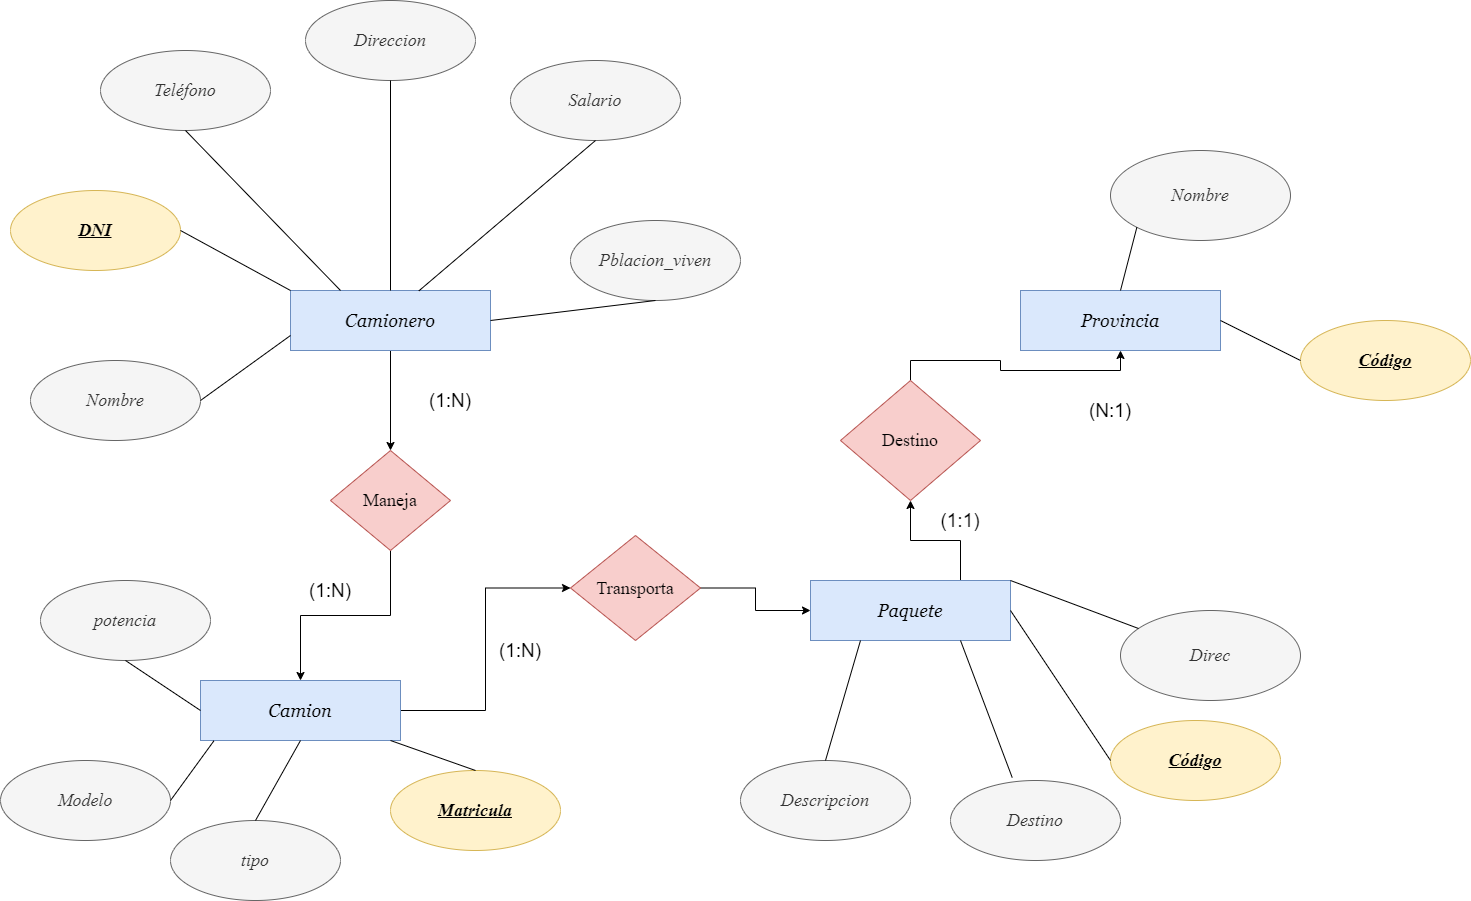
\includegraphics[width=16cm,height=10cm]{er2.png}
        \end{figure}
        \subsubsection{Diagrama Relacional}
        \begin{figure}[H]
            \centering
            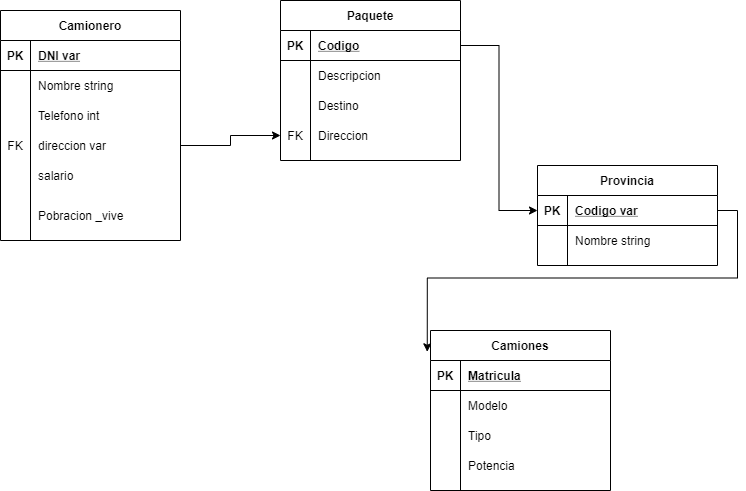
\includegraphics[width=16cm,height=10cm]{rel2.png}
        \end{figure}
        \subsubsection{Consulta de SQL}
\begin{verbatim}
CREATE DATABASE Ejercicio2_Act1;

USE Ejercicio2_Act1;

CREATE TABLE Camionero(
    DNI int primary key not null,
    Nombre varchar(50) not null,
    Telefono int not null,
    direccion varchar(255) not null,
    salario float not null,
    Población_vive varchar(50) not null
);

CREATE TABLE Paquete(
    Código int primary key not null,
    Descripcion varchar(50) not null,
    Destino varchar(255) not null,
    Dirección varchar(255) not null,
    DNI int not null,
    FOREIGN KEY (DNI) REFERENCES Camionero (DNI)
);

CREATE TABLE Provincia(
    Codigo int primary key not null,
    Nombre varchar(50) not null,
    IDPaquete int not null,
    FOREIGN KEY (IDPaquete) REFERENCES Paquete (Código)
);

CREATE TABLE Camiones(
    Matrícula int primary key not null,
    Modelo varchar(20) not null,
    Tipo varchar(20) not null,
    Potencia float not null,
    IDProvincia int not null,
    FOREIGN KEY (IDProvincia) REFERENCES Provincia (Codigo)
);
\end{verbatim}
        \subsubsection{Diagrama de SQL}
        \begin{figure}[H]
            \centering
            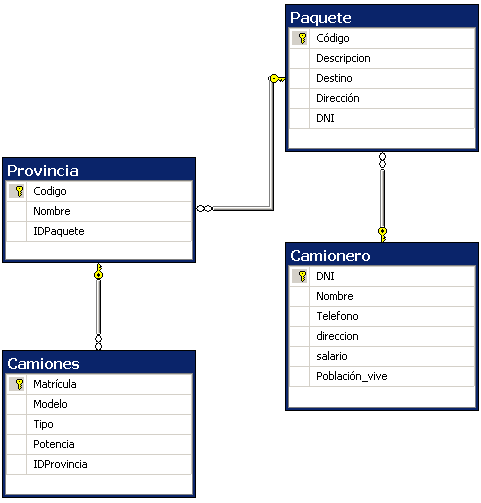
\includegraphics[width=8cm,height=10cm]{sql2.png}
        \end{figure}
        \subsubsection{Conclusión}
        \justify
        Al ser uno de los ejercicios cortos y con los diagramas hechos de antemano, no se presento mucha complicación al respecto.
        \subsection{Ejercicio 3}
        \justify
        A partir del siguiente supuesto diseñar el modelo entidad-relación. ``Se desea diseñar una base de datos para almacenar y gestionar la información
        empleada por una empresa dedicada a la venta de automóviles, teniendo en cuenta los siguientes aspectos: La empresa dispone de una serie de coches para
        su venta, Se necesita conocer la matrícula, marca y modelo; el color y el precio de venta de cada coche. Los datos que interesa conocer de cada cliente
        son el NIFm nombre, dirección, ciudad y número de teléfono: además, los clientes se diferencian por un código interno de la empresa que se incrementa
        automáticamente cuando un cliente se da de alta en ella. Un cliente puede comprar tantos coches como desee a la empresa. Un coche determinado solo puede ser comprado
        por un único cliente. El concesionario también se encarga de llevar a cabo las revisiones automáticamente por cada revisión que se haga. De cada revisión se desea saber
        si se ha hecho cambio de filtro, si se ha hecho cambio de aceite, si se ha hecho cambio de frnos u otros. Los coches pueden pasar varias revisiones en el concesionario''.
        \subsubsection{Diagrama E-R}
        \begin{figure}[H]
            \centering
            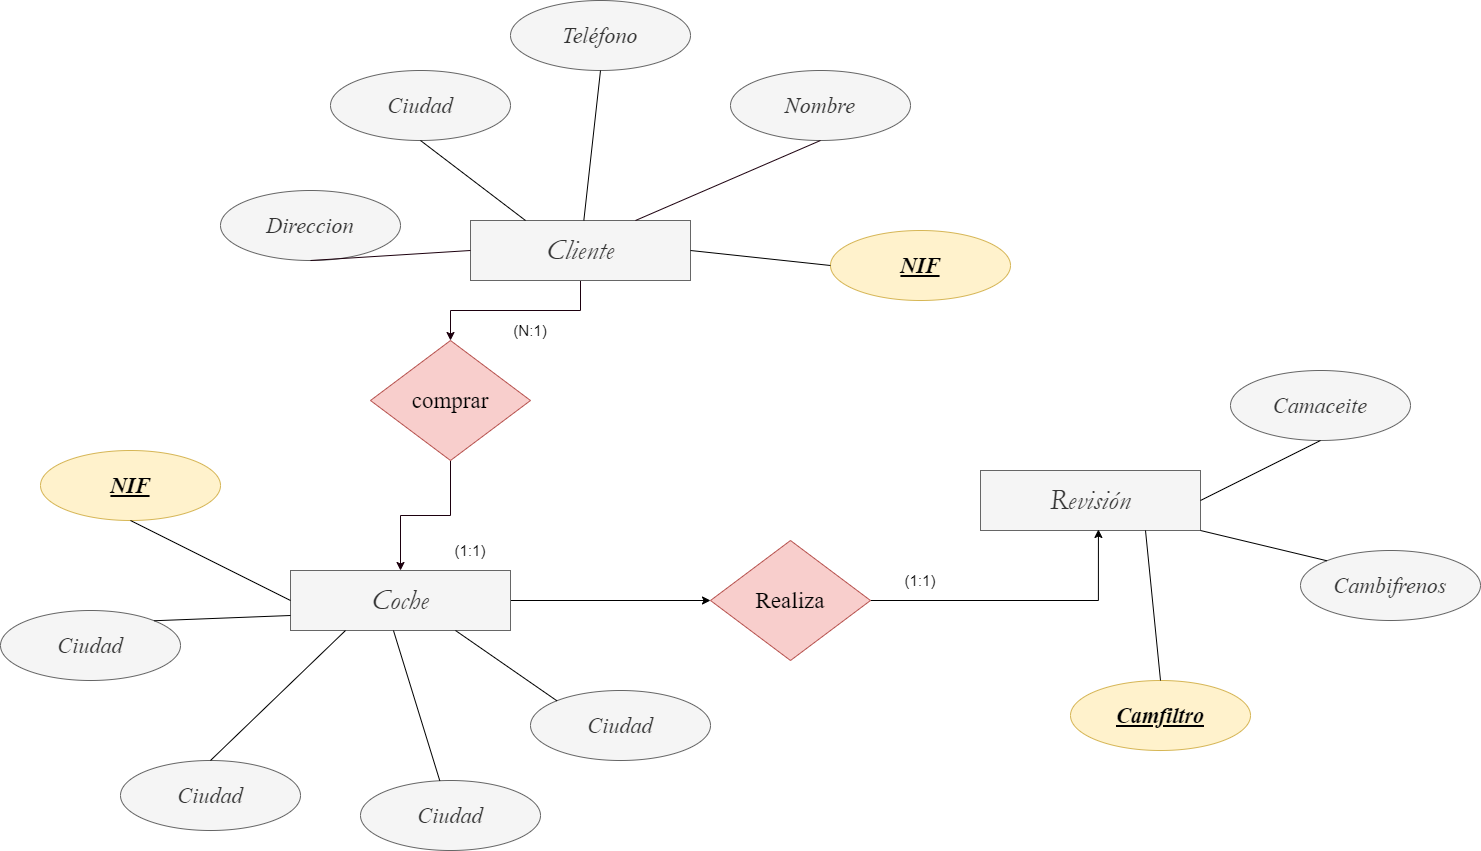
\includegraphics[width=16cm,height=10cm]{er3.png}
        \end{figure}
        \subsubsection{Diagrama Relacional}
        \begin{figure}[H]
            \centering
            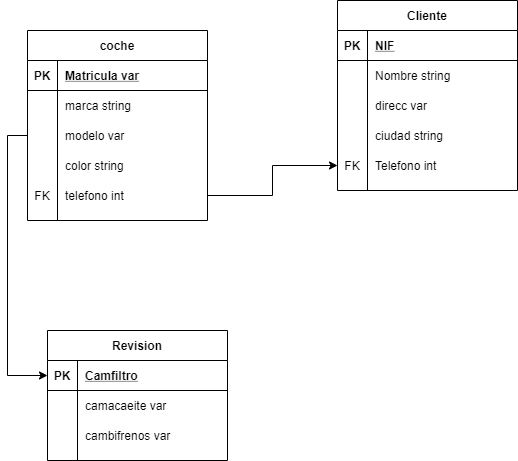
\includegraphics[width=16cm,height=10cm]{rel3.png}
        \end{figure}
        \subsubsection{Consulta de SQL}
\begin{verbatim}
CREATE DATABASE Ejercicio3_Act1;

USE Ejercicio3_Act1;

CREATE TABLE Revision(
    Camfiltro int primary key not null,
    camaceite varchar(50) not null,
    cambifrenos varchar(50) not null
);

CREATE TABLE coche(
    Matricula int primary key not null,
    marca varchar(50) not null,
    modelo varchar(20) not null,
    color varchar(20) not null,
    telefono int not null,
    Camfiltro int not null,
    FOREIGN KEY (Camfiltro) REFERENCES Revision (Camfiltro)
);

CREATE TABLE Cliente(
    NIF int primary key not null,
    Nombre varchar (50) not null,
    direcc varchar(255) not null,
    ciudad varchar(100) not null,
    Telefono int not null,
    Matricula int not null,
    FOREIGN KEY (Matricula) REFERENCES coche (Matricula)
);
\end{verbatim}
        \subsubsection{Diagrama de SQL}
        \begin{figure}[H]
            \centering
            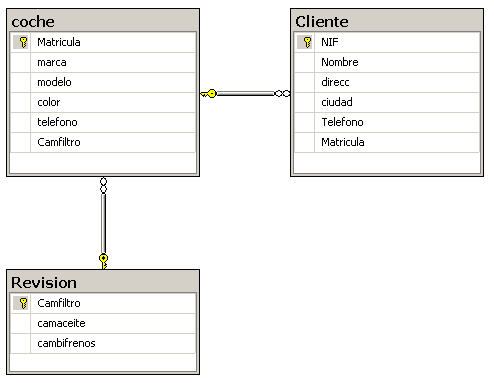
\includegraphics[width=8cm,height=8cm]{sql3.PNG}
        \end{figure}
        \subsubsection{Conclusión}
        \justify
        Similar a los anteriores, no hubo complicaciones sustanciales. Teniendo los diagramas, el planteamiento en SQL es más simple.
        \subsection{Ejercicio 4}
        \justify
        A partir del siguiente supuesto realizar el modelo entidad-relación y pasarlo a modelo relacional. ``A un concesionario de coches llegan clientes para comprar automóviles. De cada coche
        interesa saber la matrícula, modelo, marca y color. Un cliente puede comprar varios coches en el concesionario. Cuando un cliente compra un coche, se le hace una ficha en el concesionario
        con la siguiente información: dni, nombre, apellidos, dirección y teléfono. Los coches que el concesionario vende pueden ser nuevos o usados (de segunda mano). De los coches nuevos interesa
        saber el número de unidades que hay en el concesionario. De los coches viejos interesa el número de kilómetros que lleva recorridos. El concesionario también dispone de un taller en el que los
        mecánicos reparan los coches que llevan los clientes. Un mecánico repara varios coches a los largo del día, y un coche puede ser reparado por varios mecánicos. Los mecánicos tienen un dni, nombre, 
        apellidos, fecha de contratación y salario. Se desea guardar también la fecha en la que se repara cada vehículo y el número de horas que se tardó en arreglar cada automóvil''. Para el modelo entidad-
        relación resultante al modelo relacional.
        \subsubsection{Diagrama E-R}
        \begin{figure}[H]
            \centering
            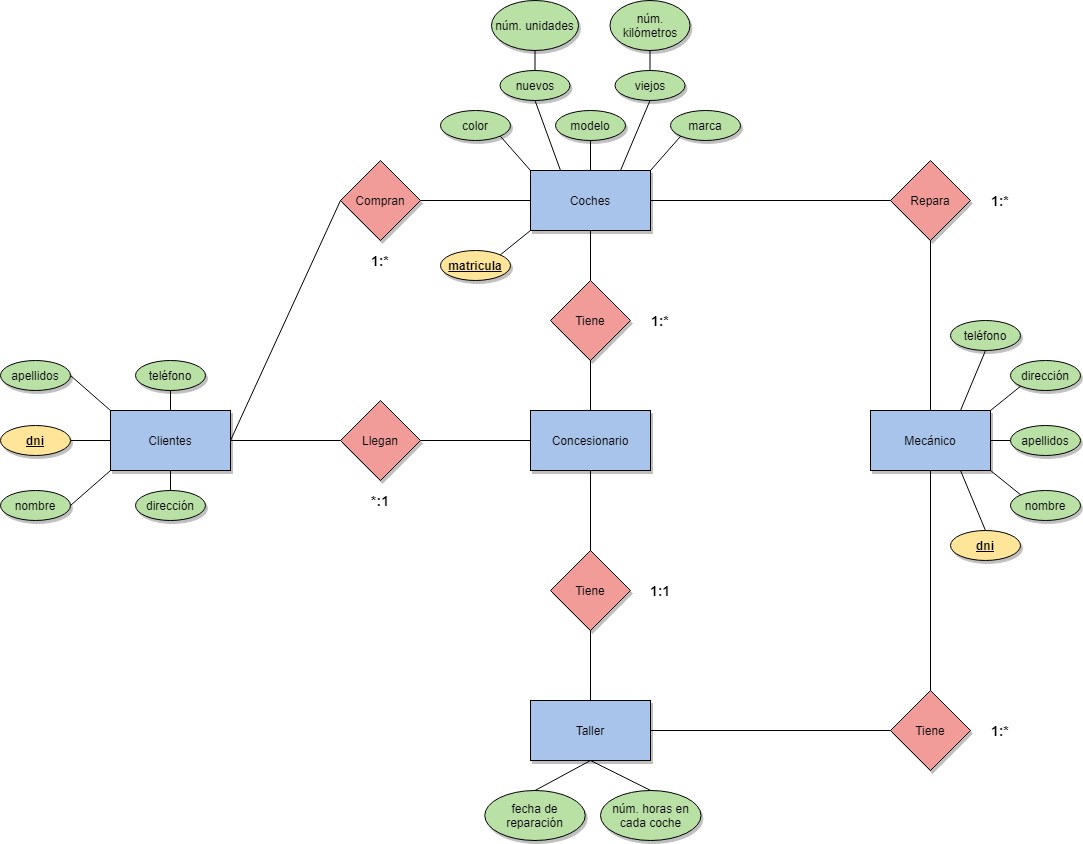
\includegraphics[width=16cm,height=10cm]{er4.png}
        \end{figure}
        \subsubsection{Diagrama Relacional}
        \begin{figure}[H]
            \centering
            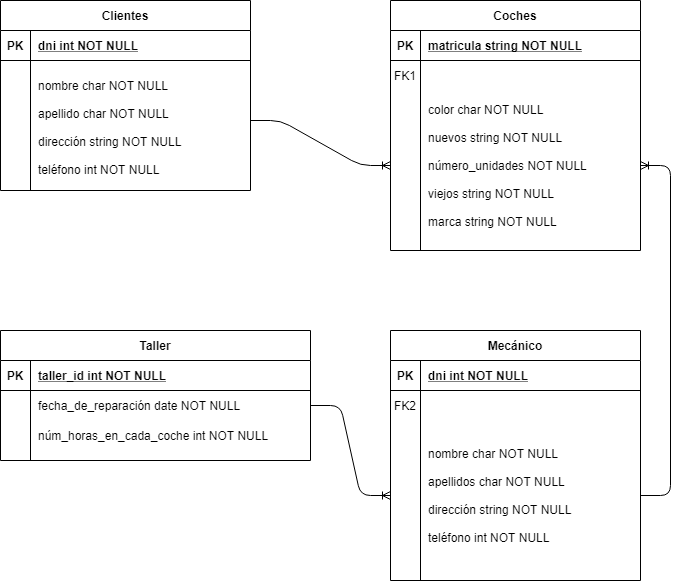
\includegraphics[width=16cm,height=10cm]{rel4.png}
        \end{figure}
        \subsubsection{Consulta de SQL}
\begin{verbatim}
CREATE DATABASE Ejercicio4_Act1;

USE Ejercicio4_Act1;

CREATE TABLE Clientes(
    dni int primary key not null,
    nombre varchar(50) not null,
    dirección varchar(255) not null,
    teléfono int not null
);

CREATE TABLE Taller(
    taller_id int primary key not null,
    fecha_de_reparación date not null,
    núm_horas_en_cada_coche int not null
);

CREATE TABLE Mecánico(
    dni int primary key not null,
    nombre varchar(50) not null,
    apellidos varchar(50) not null,
    dirección varchar(255) not null,
    teléfono int not null,
    taller_id int not null,
    FOREIGN KEY (taller_id) REFERENCES Taller (taller_id)
);

CREATE TABLE  Coches(
    matricula varchar primary key not null,
    color varchar(20) not null,
    nuevos varchar(2) not null,
    viejos varchar(2) not null,
    número_unidades int not null,
    marca varchar(10) not null,
    id_cliente int not null,
    id_mecánico int not null,
    FOREIGN KEY (id_cliente) REFERENCES Clientes (dni),
    FOREIGN KEY (id_mecánico) REFERENCES Mecánico (dni)
);
\end{verbatim}
        \subsubsection{Diagrama de SQL}
        \begin{figure}[H]
            \centering
            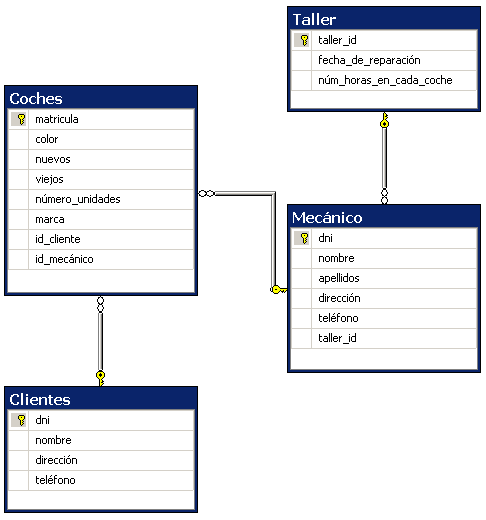
\includegraphics[width=10cm,height=10cm]{sql4.png}
        \end{figure}
        \subsubsection{Conclusión}
        \justify
        Este es uno de los ejercicios complicados debido a tener los diagramas más elaborados. Por ende se presentó dificultades para organizar todo en SQL.
        \subsection{Ejercicio 5}
        \justify
        La liga de fútbol profesional, presidida por Janito Rodríguez, ha decidido informatizar sus instalaciones creando una base de datos para guardar la información de los partidos que se juegan en la liga.
        Se desea guardar en primer lugar los datos de los jugadores. De cada jugador se quiere guardar el nombre, fecha de nacimiento y posición en la que juega (portero, defensa, centrocampísta...). Cada jugador
        tiene un código de jugador que lo identifica de manera única. De cada uno de los equipos de la liga es necesario registrar el nombre del equipo, nombre del estadio en el que juega, el aforo que tiene, el año
        de fundación del equipo y la ciudad de la que es el equipo. Cada equipo también tiene un código que lo identifica de manera única. Un jugador solo puede pertenecer a un único equipo. De cada partido que los equipos
        de la liga juegan hay que registrar la fecha en la que se juega el partido, los goles que ha metido el equipo de casa y los goles que ha metido el equipo de fuera. Cada partido tendrá un código numérico para identificar
        el partido. También se quiere llevar un recuento de los goles que hay en cada partido. Se quiere almacenar el minuto en el que se realiza el gol y la descripción del gol. Un partido tiene varios goles y un jugador
        puede meter varios goles en un partido. Por último se quiere almacenar, en la base de datos, los datos de los presidentes de los equipos de fútbol (dni, nombre, apellidos, fecha de nacimiento, equipo del que es presidente
        y año en el que fue elegido presidente). Un equipo de fútbol tan sólo puede tener un presidente, y una persona sólo puede ser presidente de un equipo de la liga. Parar el modelo entidad-relación resultante al modelo relacional.
        \subsubsection{Diagrama E-R}
        \begin{figure}[H]
            \centering
            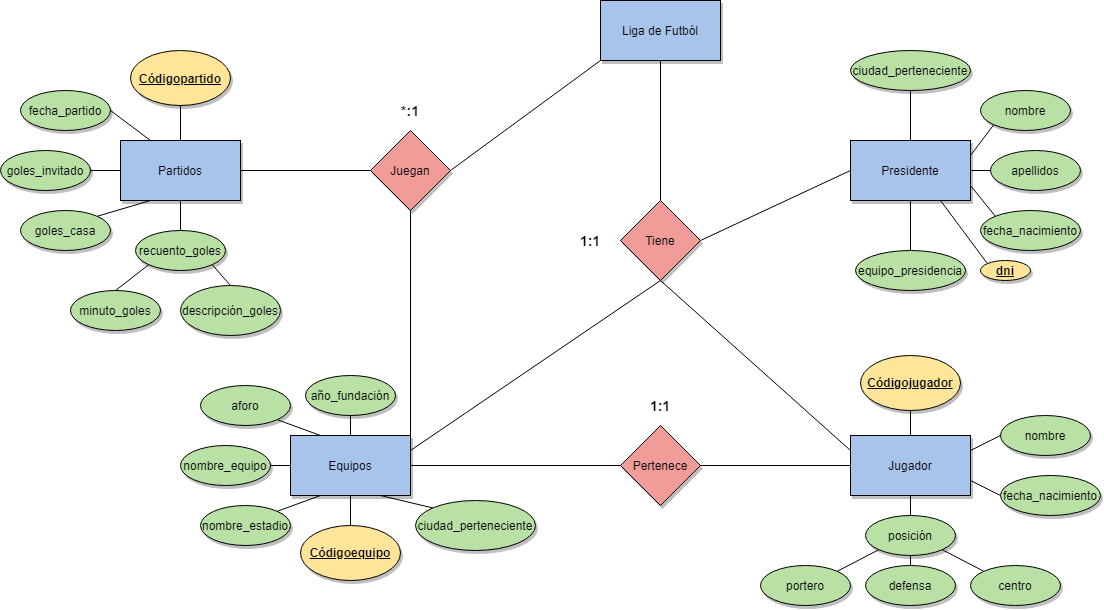
\includegraphics[width=16cm,height=10cm]{er5.png}
        \end{figure}
        \subsubsection{Diagrama Relacional}
        \begin{figure}[H]
            \centering
            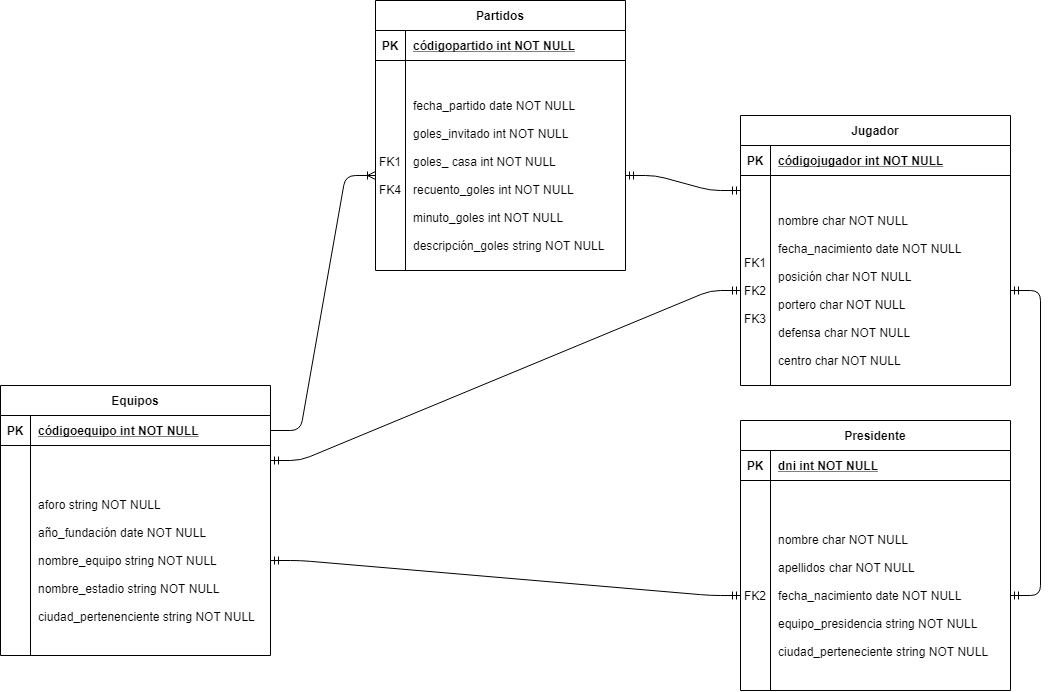
\includegraphics[width=16cm,height=10cm]{rel5.png}
        \end{figure}
        \subsubsection{Consulta de SQL}
\begin{verbatim}
CREATE DATABASE Ejercicio5_Act1;

USE Ejercicio5_Act1;

CREATE TABLE Equipos(
    códigoequipo int primary key not null,
    aforo varchar(50) not null,
    año_fundación date not null,
    nombre_equipo varchar not null,
    nombre_estadio varchar not null,
    ciudad_perteneciente varchar not null
);

CREATE TABLE Presidente(
    dni int primary key not null,
    nombre varchar(50) not null,
    apellidos varchar(50) not null,
    fecha_nacimiento date not null,
    equipo_presidencia varchar not null,
    ciudad_perteneciente varchar not null,
    códigoequipo int not null,
    FOREIGN KEY (códigoequipo) REFERENCES Equipos (códigoequipo)
);

CREATE TABLE Partidos(
	códigopartido int primary key not null,
    fecha_partido date not null,
    goles_invitado int not null,
    goles_casa int not null,
    recuento_goles int not null,
    minuto_goles int not null,
    descripción_goles varchar not null,
    códigoequipo int not null,
    FOREIGN KEY (códigoequipo) REFERENCES Equipos (códigoequipo)
);

CREATE TABLE Jugador(
    códigojugador int primary key not null,
    nombre varchar(50) not null,
    fecha_nacimiento date not null,
    posición varchar(50) not null,
    portero varchar(2) not null,
    defensa varchar(2) not null,
    centro varchar(2) not null,
    códigoequipo int not null,
    códigopartido int not null,
    dni_presidente int not null,
    FOREIGN KEY (códigoequipo) REFERENCES Equipos (códigoequipo),
    FOREIGN KEY (códigopartido) REFERENCES Partidos (códigopartido),
    FOREIGN KEY (dni_presidente) REFERENCES Presidente (dni)
);
\end{verbatim}
        \subsubsection{Diagrama de SQL}
        \begin{figure}[H]
            \centering
            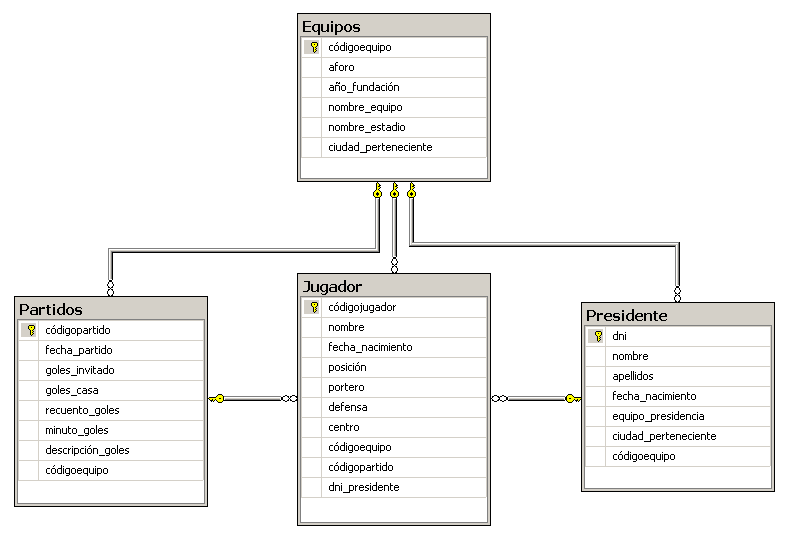
\includegraphics[width=12cm,height=12cm]{sql5.png}
        \end{figure}
        \subsubsection{Conclusión}
        \justify
        A pesar de tener el diagrama relación extenso, su implementación a SQL es bastante sencilla. Como en ejercicios anteriores, no existen muchas complicaciones mas allá de los errores de redacción.
        \subsection{Ejercicio 6}
        \justify
        Una agencia de viajes desea informatizar toda la gestión de los viajeros que acuden a la agencia y los viajes que estos realizan. Tras ponernos en contacto con la agencia, ésta nos proporciona la siguiente información. ``La agencia 
        desea guardar la siguiente información de los viajeros: dni, nombre, dirección y teléfono. De cada uno de los viajes que maneja la agencia interesa guardar el código de viaje, número de plazas, fecha en la que se realiza el viaje y
        otros datos. Un viajero puede realizar tantos viajes como desee con la agencia, Un viaje determinado sólo puede ser cubierto por un viajero. Cada viaje realizado tiene un destino y un lugar de origen. De cada uno de ellos se quiere almacenar
        el código, nombre y otros datos que puedan ser de interés. Un viaje tiene un único lugar de destino y un único lugar de origen''. Realizar el modelo E-R.
        \subsubsection{Diagrama E-R}
        \begin{figure}[H]
            \centering
            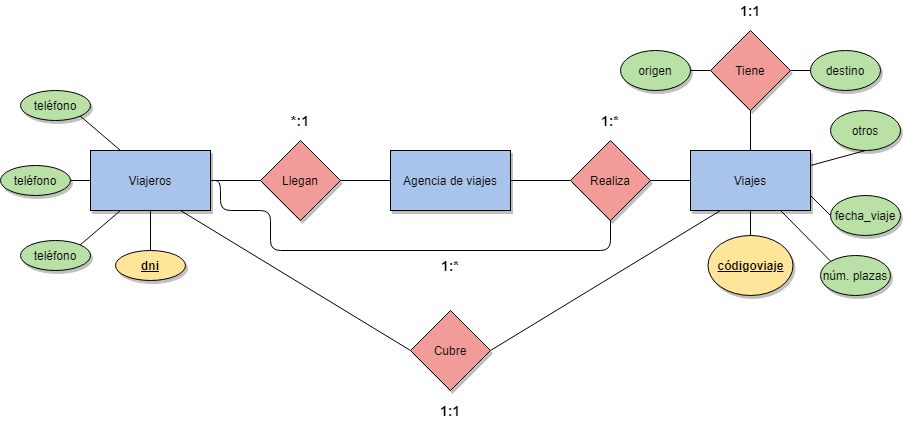
\includegraphics[width=16cm,height=10cm]{er6.png}
        \end{figure}
        \subsubsection{Diagrama Relacional}
        \begin{figure}[H]
            \centering
            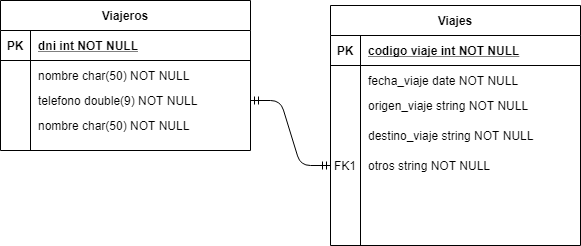
\includegraphics[width=16cm,height=10cm]{rel6.png}
        \end{figure}
        \subsubsection{Consulta de SQL}
\begin{verbatim}
CREATE DATABASE Ejercicio6_Act1;

USE Ejercicio6_Act1;

CREATE TABLE Viajeros(
    dni int primary key not null,
    nombre varchar(50) not null,
    telefono int not null,
);

CREATE TABLE Viajes(
    código_viaje int primary key not null,
    fecha_viaje date not null,
    origen_viaje varchar not null,
    destino_viaje varchar not null,
    otros varchar not null,
    dni int not null,
    FOREIGN KEY (dni) REFERENCES Viajeros (dni)
);
\end{verbatim}
        \subsubsection{Diagrama de SQL}
        \begin{figure}[H]
            \centering
            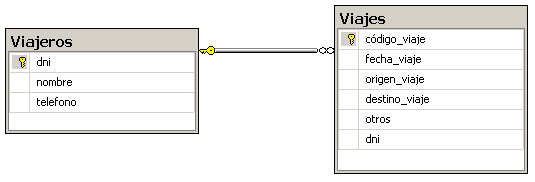
\includegraphics[width=12cm,height=8cm]{sql6.PNG}
        \end{figure}
        \subsubsection{Conclusión}
        \justify
        Este fue el ejercicio más sencillo de todos. Debido a que su diagrama E-R solo contiene dos relaciones, la implementación en SQL fue muy simple.
        \subsection{Ejercicio 7}
        \justify
        Se quiere modelar la realidad relativa a una clínica odontológica.
        \subsubsection{Diagrama E-R}
        \begin{figure}[H]
            \centering
            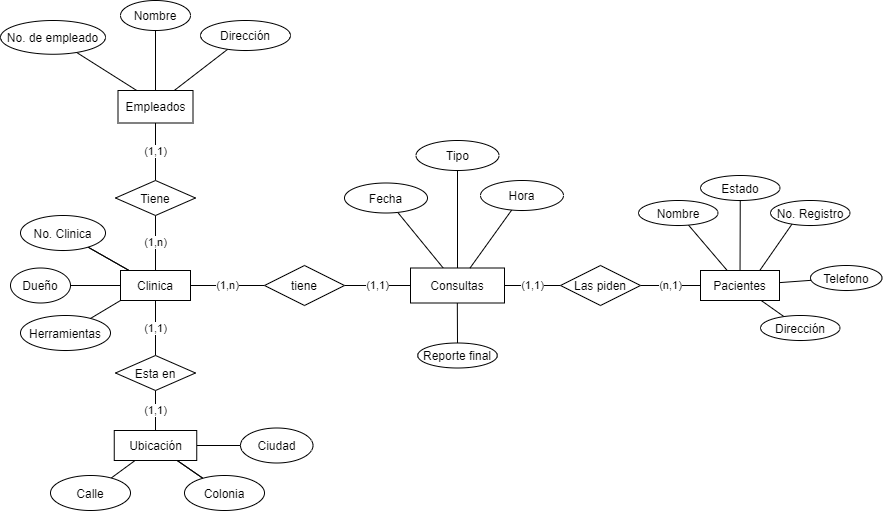
\includegraphics[width=16cm,height=10cm]{er7.png}
        \end{figure}
        \subsubsection{Diagrama Relacional}
        \begin{figure}[H]
            \centering
            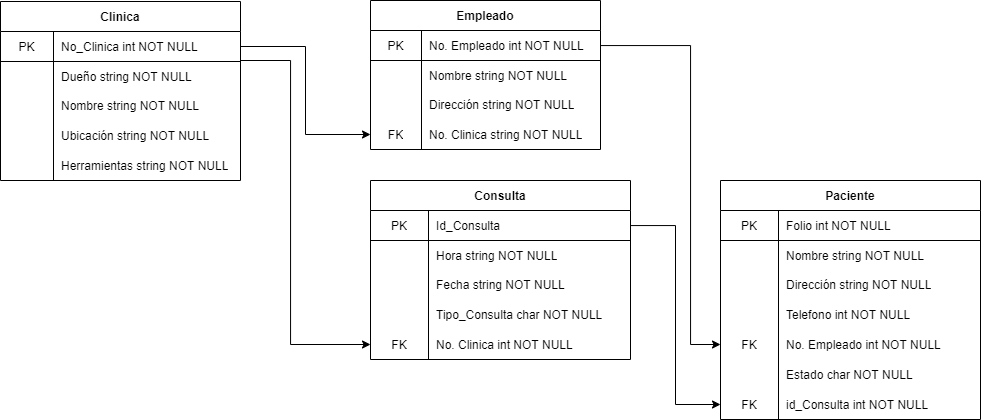
\includegraphics[width=16cm,height=10cm]{rel7.png}
        \end{figure}
        \subsubsection{Consulta de SQL}
\begin{verbatim}
CREATE DATABASE Ejercicio7_Act1;

USE Ejercicio7_Act1;

CREATE TABLE Clinica(
    No_Clinica int primary key not null,
    Dueño varchar not null,
    Nombre varchar not null,
    Ubicación varchar not null,
    Herramientas varchar not null
);

CREATE TABLE Empleado(
    No_Empleado int primary key not null,
    Nombre varchar not null,
    Dirección varchar not null,
    No_Clínica int not null,
    FOREIGN KEY (No_Clínica) REFERENCES Clinica (No_Clinica)
);

CREATE TABLE Consulta(
    id_Consulta int primary key not null,
    Hora varchar not null,
    Fecha varchar not null,
    Tipo_Consulta varchar(50) not null,
    No_Clínica int not null,
    FOREIGN KEY (No_Clínica) REFERENCES Clinica (No_Clinica)
);

CREATE TABLE Paciente(
    Folio int primary key not null,
    Nombre varchar not null,
    Dirección varchar not null,
    Telefono int not null,
    Estado varchar(50) not null,
    No_Empleado int not null,
    id_Consulta int not null,
    FOREIGN KEY (No_Empleado) REFERENCES Empleado (No_Empleado),
    FOREIGN KEY (id_Consulta) REFERENCES Consulta (id_COnsulta)
);
\end{verbatim}
        \subsubsection{Diagrama de SQL}
        \begin{figure}[H]
            \centering
            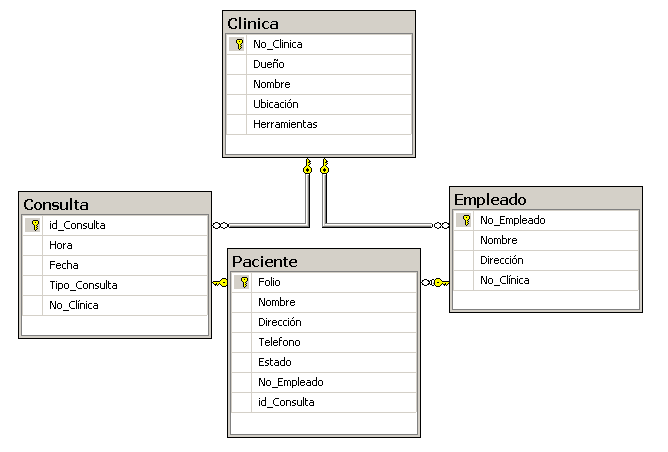
\includegraphics[width=12cm,height=10cm]{sql7.PNG}
        \end{figure}
        \subsubsection{Conclusión}
        \justify
        En lo que cabe de su creación, como solo se provió de una instrucción muy vaga, se vió en la necesidad de improvisar los posibles diagramas relacional y E-R para aplicar el resto de implementaciones.
        \subsection{Ejercicio 8}
        \justify
        Las sedes olímpicas se dividen en complejos deportivos. Los complejos deportivos se subdividen en aquellos en los que se desarrolla un único deporte y en los polideportivos. Los complejos polideportivos tienen áreas designadas para cada deporte
        con un indicador de localización (ejemplo: centro, esquinaNE, etc.). Un complejo tiene una localización, un jefe de organización individual y un área total ocupada. Los dos tipos de complejos (deporte único y polideportivo) tendrán diferentes tipos de información.
        Para cada tipo de sesde, se conservará el número de complejos junto con su presupuesto aproximado. Cada complejo celebra una serie de eventos (ejemplo: la pista del estadio puede celebrar muchar carreras distintas). Para cada evento está prevista una fecha,
        duración, número de participantes, número de comisarios. Una lista de todos los comisarios se conservará junto con la lista de los eventos en los que esté involucrado cada comisario ya sea cumpliendo la tarea de juez u observador. Tanto para cada evento como para el
        manteniemiento se necesitará cierto equipamiento (ejemplo: arcos, pértigas, barras paralelas, etc.).
        \subsubsection{Diagrama E-R}
        \begin{figure}[H]
            \centering
            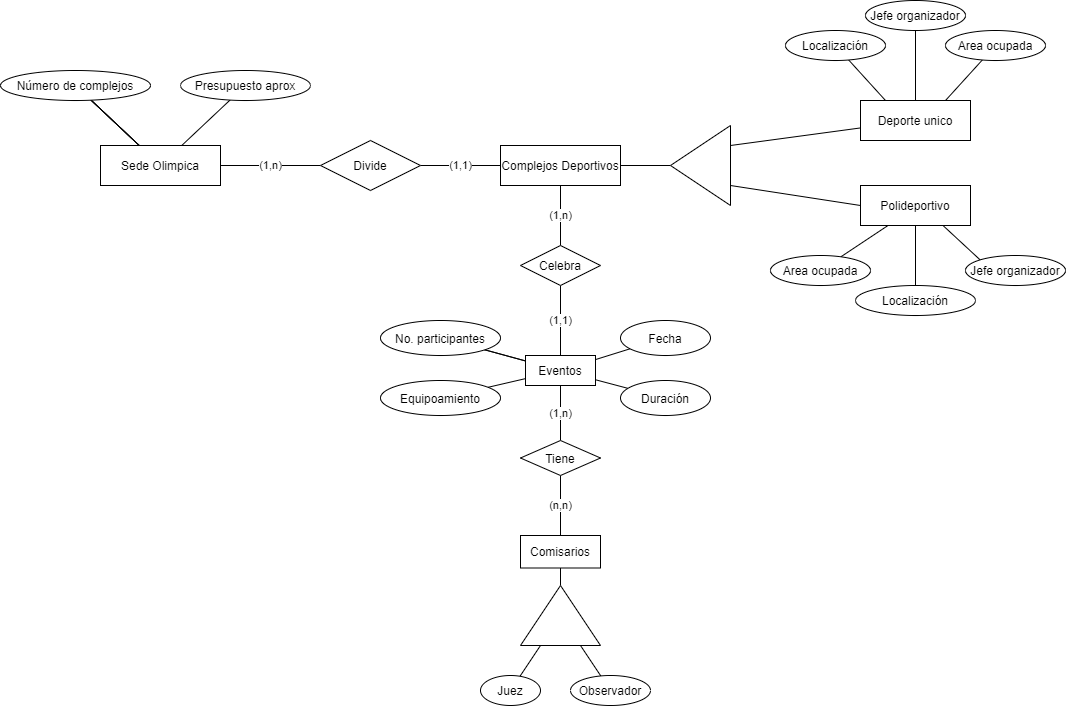
\includegraphics[width=16cm,height=10cm]{er8.png}
        \end{figure}
        \subsubsection{Diagrama Relacional}
        \begin{figure}[H]
            \centering
            \includegraphics[width=16cm,height=10cm]{rel8.jpg}
        \end{figure}
        \subsubsection{Consulta de SQL}
\begin{verbatim}
CREATE DATABASE Ejercicio8_Act1;

USE Ejercicio8_Act1;

CREATE TABLE Sede_Olimpica(
    Id_Sede int primary key not null,
    Presupuesto int not null,
    Nombre varchar not null
);

CREATE TABLE Complejo_Deportivo(
    Id_Complejo int primary key not null,
    Ubicación varchar not null,
    Area float not null,
    T_Deporte varchar(50) not null,
    Id_Sede int not null,
    FOREIGN KEY (Id_Sede) REFERENCES Sede_Olimpica (Id_Sede)
);

CREATE TABLE Evento(
    Id_Evento int primary key not null,
    Nombre varchar not null,
    Duración int not null,
    Id_Complejo int not null,
    FOREIGN KEY (Id_Complejo) REFERENCES Complejo_Deportivo (Id_Complejo)
);

CREATE TABLE Encargado_Evento(
    Id_Comisario int primary key not null,
    Nombre varchar not null,
    Posición varchar(50) not null,
    Id_Evento int not null,
    FOREIGN KEY (Id_Evento) REFERENCES Evento (Id_Evento)
);
\end{verbatim}
        \subsubsection{Diagrama de SQL}
        \begin{figure}[H]
            \centering
            \includegraphics[width=10cm,height=10cm]{sql8.PNG}
        \end{figure}
        \subsubsection{Conclusión}
        \justify
        Similar a los ejercicios anteriores, su implementación no causo problema ya que solo se presentó una llave primaria por cada relación.
        \subsection{Ejercicio 9}
        \justify
        El sistema debe memorizar todos los encuentros que se han desarrollado desde que existe el torneo, así como las siguientes características de estos.\\
        \textbf{Descripción:} El Grand Slam se compone de cuatro torneas anuales que se celebran en Gran Bretaña, Estados Unidos, Francia y Australia. En cada país se pueden desarrollar en distintos lugares
        (p- ej., en EE.UU. puede desarrikkarse eb Forest Hill o en Flashing Meadows). Cada partido tiene asociado un premio de consolación para el perdedor que dependerá de la fase en que se encuentre el torneo (p. ej., el perdedor octavos de final puede ganar 5,000 dólares).
        El ganador de la final recibirá el premio correspondiente al torneo. Cada torneo tiene cienco modalidades: Indivual masculino, individual femenino, dobles masculino, dobles femenino y dobles mixtos. También hay que tener en cuenta la nacionalidad de un jugador, de forma que
        este puede ser apátrida o tener varias nacionalidades.\\
        \textbf{Resultados a considerar:} Elsistema debe dar respuesta a las siguentes preguntas:
        \begin{enumerate}
            \item Dado un año y un torneo, composición y resultado de los partidos.
            \item Lista de árbitros que participaron en el torneo.
            \item Ganancias percibidas en premios por un jugador a lo largo del torneo.
            \item Lista de entrenadores que han entrenado a un jugador a lo largo del torneo y fechas en las que lo hizo.
        \end{enumerate} 
        Ejemplos de acceso a la base de datos:
        \begin{enumerate}
            \item Connors ganó Gerulaitis en Roland Garros en 1979 en cuartos de final en individuales masculinos por 6-3 4-3/7-5 6-0.
            \item El señor Wlkinson árbitro ese partido.
            \item Alemanio ha ganado dos veces las individuales masculinas de Wimbledon. Borg ha ganado 2,000,000 de dólares a lo largo de su participación en el Grand Slam.
            \item El ganador de Roland Garros de 1987 ganó 20,000 dólares.
            \item Noah ha jugado cuatro veces en dobles mixtos con Mandlikova.
        \end{enumerate}
        \subsubsection{Diagrama E-R}
        \begin{figure}[H]
            \centering
            \includegraphics[width=16cm,height=10cm]{er9.png}
        \end{figure}
        \subsubsection{Diagrama Relacional}
        \begin{figure}[H]
            \centering
            \includegraphics[width=16cm,height=10cm]{rel9.jpg}
        \end{figure}
        \subsubsection{Consulta de SQL}
\begin{verbatim}
CREATE DATABASE Ejercicio9_Act1;

USE Ejercicio9_Act1;

CREATE TABLE Grand_Slam(
    Id_Torneo int primary key not null,
    Nombre string not null,
    Año int not null
);

CREATE TABLE Torneo(
    Ubicación string primary key not null,
    Premio_C float not null,
    Premio_final float not null,
    Id_Torneo int not nullm
    FOREIGN KEY (Id_Torneo) REFERENCES Grand_Slam (Id_Torneo)
);

CREATE TABLE Modalidad(
    Modalidad string primary key not null,
    Nombre string not null,
    Ubicación string not null,
    FOREIGN KEY (Ubicación) REFERENCES Torneo (Ubicación)
);

CREATE TABLE Jugadores(
    No_Jugador int not null,
    Nombre string not null,
    Ganancia float not null,
    Ubicación string not null,
    Modalidad string not null,
    FOREIGN KEY (Ubicación) REFERENCES Torneo (Ubicación),
    FOREIGN KEY (Modalidad) REFERENCES Modalidad (Modalidad)
);

CREATE TABLE Entrenado(
    id_Entrenador int primary key not null,
    Nombre string not null,
    Fecha_Entreno string not null,
    No_Jugador int not null,
    FOREIGN KEY (No_Jugador) REFERENCES Jugadores (No_Jugador)
);
\end{verbatim}
        \subsubsection{Diagrama de SQL}
        \begin{figure}[H]
            \centering
            \includegraphics[width=10cm,height=10cm]{sql9.PNG}
        \end{figure}
        \subsubsection{Conclusión}
        \justify
        Fue uno de los diagramas más complejos a implementar debido a tener muchas llaves primarias, lo que la mala implementación de las mismas causa estragos en la ejecución de las consultas de SQL.
        \section{Actividad: U5T2 Ejercicio Individual Algebra Relacional}
        \justify
        \subsection{Consulta de SQL}
\begin{verbatim}
CREATE DATABASE actividad_ind_AR;

USE actividad_ind_AR;

CREATE TABLE Cliente (
N_Cliente int primary key not null,
Nombre varchar (100) not null,
Direccion varchar (50) not null,
Telefono varchar (16) not null,
Poblacion varchar (30) not null);

CREATE TABLE Producto (
Cod_Producto int primary key not null,
Descripcion varchar (255) not null,
Precio float not null);

CREATE TABLE Factura (
N_Factura int primary key not null,
Fecha smalldatetime not null,
Pagada bit not null,
N_Cliente int not null,
FOREIGN KEY (N_Cliente) REFERENCES Cliente (N_Cliente));

CREATE TABLE Venta (
ID_Venta int primary key not null,
Cantidad int not null,
N_Factura int not null,
Cod_Producto int not null,
FOREIGN KEY (N_Factura) REFERENCES Factura (N_Factura),
FOREIGN KEY (Cod_Producto) REFERENCES Producto (Cod_Producto));
\end{verbatim}
        \subsection{Diagrama de SQL}
        \begin{figure}[H]
            \centering
            \includegraphics[width=10cm,height=10cm]{sql_u5t2.PNG}
        \end{figure}
        \subsection{Conclusión}
        \justify
        Similar a consultas anteriores, por ser implicitamente condicional, facilita bastante la consulta en SQL.
        \section{Actividad: U5T3 A-R Equipos (Ejercicio 1: Operaciones de proyección y selección)}
        \justify
        Una empresa de venta de música on-line necesita diseñar una base de datos para modelar las tarjetas
        de crédito de sus clientes. La información se organiza de la siguiente manera en la relación Tarjeta:
        \begin{table}[H]
            Tarjeta\\
            \begin{tabular}{|c|c|c|c|c|}
            \hline
            \textbf{Cliente} & \textbf{Nombre}  & \textbf{Número} & \textbf{Vencimiento} & \textbf{BancoEmisor} \\ \hline
            Caetano Veloso   & VISA             & 9876 1234       & 08/2013              & Banco Nación         \\ \hline
            Caetano Veloso   & American Express & 1357 9753       & 12/2014              & Banco Santader Río   \\ \hline
            Caetano Veloso   & Mastercard       & 2468 9321       & 07/2014              & Banco Francés        \\ \hline
            Rubén Rada       & VISA             & 3546 1212       & 09/2013              & Banco Francés        \\ \hline
            Paco de Lucía    & Mastercard       & 1035 9857       & 11/2015              & Banco Credicoop      \\ \hline
            Silvio Rodriguéz & Tarjeta Naranja  & 8345 6723       & 12/2015              & Banco Nación         \\ \hline
            \end{tabular}
        \end{table}
        \subsection{Consulta de SQL}
\begin{verbatim}
CREATE DATABASE Algebrateam1;

USE Algebrateam1;
    
CREATE TABLE Tarjeta (
Numero int primary key not null,
Cliente varchar (100) not null,
Nombre varchar (30) not null,
Vencimiento smalldatetime not null,
BancoEmisor varchar (50) not null);
\end{verbatim}
        \subsection{Diagrama de SQL}
        \begin{figure}[H]
            \centering
            \includegraphics[width=6cm,height=6cm]{sql_u5t3_1.PNG}
        \end{figure}
        \subsection{Conclusión}
        \justify
        No generó complicaciones al reutilizar estructuras similares.
        \section{Actividad: U5T3 A-R Equipos (Ejercicio 2: Operaciones de Producto y \emph{Join} Natural)}
        \justify
        Considerar las relaciones \emph{Alumno, Cursa, Materia y Profesor}
        \begin{table}[H]
            Alumno\\
            \begin{tabular}{|c|c|c|c|}
            \hline
            \textbf{NombreAlumno} & \textbf{\#Alumno} & \textbf{FechaNacAlu} & \textbf{LegajoTutor} \\ \hline
            Sheldon Cooper        & 3110             & 1993                 & 162                  \\ \hline
            Raj Kothrappali       & 4220             & 1991                 & 078                  \\ \hline
            Leonard Hofstadter    & 4221             & 1988                 & 052                  \\ \hline
            Howard Wolowitz       & 5110             & 1990                 & 162                  \\ \hline
            \end{tabular}
        \end{table}
        \begin{table}[H]
            Cursa\\
            \begin{tabular}{|c|c|c|}
            \hline
            \textbf{\#Alumno} & \textbf{CodigoMateria}         & \textbf{Nota} \\ \hline
            3110             & Bases de Datos                 & 5             \\ \hline
            3110             & Introducción a la Programación & 6             \\ \hline
            3110             & Programación con Objetos I     & 7             \\ \hline
            4221             & Bases de Datos                 & 8             \\ \hline
            4220             & Bases de Datos                 & 4             \\ \hline
            \end{tabular}
        \end{table}
        \begin{table}[H]
            Materia\\
            \begin{tabular}{|c|c|c|}
            \hline
            \textbf{CodigoMateria}         & \textbf{NotaMinimaCursada} & \textbf{NotaMinimaPromoción} \\ \hline
            Bases de Datos                 & 4                          & 7                            \\ \hline
            Introducción a la Programación & 4                          & 7                            \\ \hline
            Programación con Objetos I     & 6                          & 9                            \\ \hline
            \end{tabular}
        \end{table}
        \begin{table}[H]
            Profesor\\
            \begin{tabular}{|c|c|c|}
            \hline
            \textbf{Legajo} & \textbf{NombreProfesor} & \textbf{FechaNacProfesor} \\ \hline
            078             & Stephen Hawking         & 1960                      \\ \hline
            162             & Alan Kay                & 1955                      \\ \hline
            052             & John Hughes             & 1970                      \\ \hline
            191             & Steve Jobs              & 1970                      \\ \hline
            \end{tabular}
            \end{table}
        \subsection{Consulta de SQL}
\begin{verbatim}
CREATE DATABASE Algebrateam2;

USE Algebrateam2;

CREATE TABLE Profesor (
Legajo int primary key not null,
NombreProfesor varchar (100) not null,
FechaNacProfesor smalldatetime not null);

CREATE TABLE Materia (
CodigoMateria int primary key not null,
NombreMateria varchar (30) not null,
NotaMinimaCursada char not null,
NotaMinimaPromocion char not null);

CREATE TABLE Alumno (
Num_Alumno int primary key not null,
NombreAlumno varchar (100) not null,
FechaNacAlu smalldatetime not null,
Legajo int not null,
FOREIGN KEY (Legajo) REFERENCES Profesor (Legajo));

CREATE TABLE Cursa (
Nota char not null,
Num_Alumno int not null,
CodigoMateria int not null,
FOREIGN KEY (Num_Alumno) REFERENCES Alumno (Num_Alumno),
FOREIGN KEY (CodigoMateria) REFERENCES Materia (CodigoMateria));
\end{verbatim}
        \subsection{Diagrama de SQL}
        \begin{figure}[H]
            \centering
            \includegraphics[width=10cm,height=10cm]{sql_u5t3_2.PNG}
        \end{figure}
        \subsubsection{Conclusión}
        \justify
        Similar a los ejercicios anteriores, no hay complicaciones aparentes.
        \section{Actividad: U5T3 A-R Equipos (Ejercicio 3: Operaciones de conjuntos)}
        \justify
        Sean las relaciones de \emph{Boca y River} que representan las estadísticas de Boca y River en los 4 primeros partidos del campeonato inicial de fútbol, considerando
        que el \emph{dominio} son los números del 1 al 30 para todos los atributos.
        \begin{table}[H]
            \(R_1\)\\
            \begin{tabular}{|c|c|c|}
            \hline
            \textbf{Goles} & \textbf{Tiros al Arco} & \textbf{Corners} \\ \hline
            0              & 5                      & 10               \\ \hline
            2              & 4                      & 6                \\ \hline
            3              & 10                     & 12               \\ \hline
            3              & 9                      & 14               \\ \hline
            \end{tabular}
        \end{table}
        \begin{table}[H]
            \(R_2\)\\
            \begin{tabular}{|c|c|c|}
            \hline
            \textbf{Goles} & \textbf{Tiros al Arco} & \textbf{Corners} \\ \hline
            1              & 9                      & 10               \\ \hline
            2              & 4                      & 6                \\ \hline
            4              & 8                      & 8                \\ \hline
            3              & 10                     & 12               \\ \hline
            \end{tabular}
            \end{table}
        \subsection{Consulta de SQL}
\begin{verbatim}
CREATE DATABASE Algebrateam3;
    
USE Algebrateam3;
    
CREATE TABLE R1 (
Goles char not null,
TiroArco tinyint not null,
Corners tinyint not null);

CREATE TABLE R2 (
Goles char not null,
TiroArco tinyint not null,
Corners tinyint not null); 
\end{verbatim}   
        \subsection{Diagrama de SQL}
        \begin{figure}[H]
            \centering
            \includegraphics[width=12cm,height=8cm]{sql_u5t3_3.PNG}
        \end{figure}
        \subsection{Conclusión}
        \justify
        Como ya se provee de las tablas, solo se replican en SQL.
        \section*{Conclusión general}
        \justify
        El compendio selecto de estos trabajos denota la importancia de lo visto en la materia como parte relevante de la carrera de Sistemas Computacionales.
        Poder hacer este respaso refuerza lo aprendido y agrega un cierre sólido a la materia y al semestre.

    \end{justify}
\end{document}